%=========================================================
\chapter{Modelo dinámico}	
\label{cap:modDinamico}

El presente capítulo describe el modelo dinámico de nuestro sistema propuesto. En este se explican y representan las interacciones entre los actores y las funcionalidades del sistema estructurando la información necesaria para comprender su funcionamiento y diseño para asegurar una implementación coherente y funcional.

En primer lugar, se describe la notación empleada para los diagramas de casos de uso, seguida de una pequeña explicación de porque decidimos establecer ciertos casos como necesarios y otros como no necesarios. Posteriormente, se introduce el diagrama de estructura de usuarios, que organiza a los actores según sus roles, después se describirán los actores que participaran en el sistema y se establecen sus responsabilidades y procesos. A partir de esto, se presentan los diagramas de casos de uso para los sistemas móvil y web, destacando las funcionalidades específicas de cada sistema. Finalmente, se proporciona una descripción exhaustiva de los casos de uso seleccionados como necesarios.

\section{Notación}

%\newpage

\begin{figure}[htbp!]
	\begin{center}
		\fbox{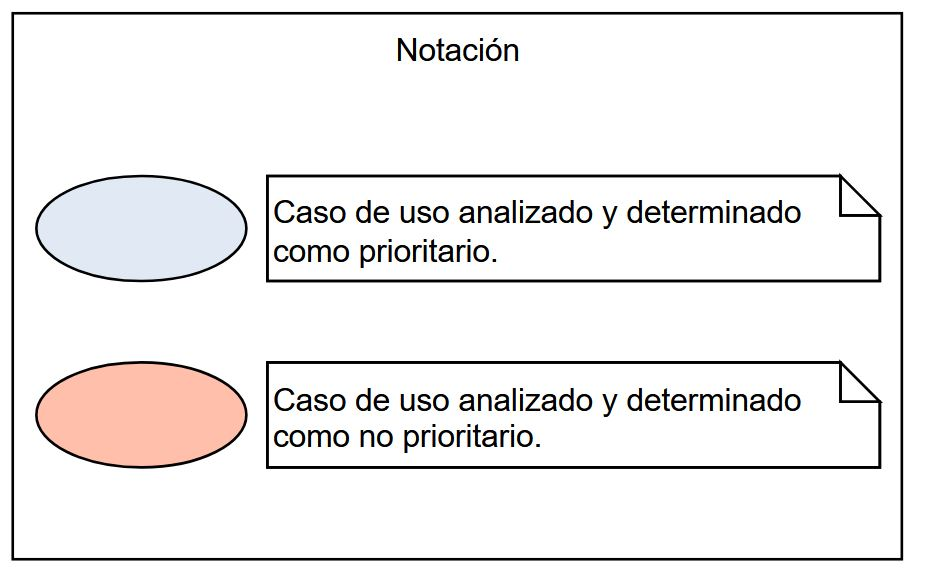
\includegraphics[width=.35\textwidth]{images/Notacion}}
		\caption{Análisis de viabilidad de los casos de uso.}
		\label{fig:Notacion}
	\end{center}
\end{figure}

Ahora comenzaremos con la explicación de la notación usada para el diagrama de casos de uso. En la figura \ref{fig:Notacion} se puede ver la notación usada para el diagrama de casos de uso, en este se puede observar que se usaron 2 colores para clasificarlos; los casos de uso de color azul fueron analizados y determinados como prioritarios y los casos de uso de color rojo fueron analizados y determinados como no prioritarios.

Decidimos determinar como casos de uso prioritarios a todos los casos del sistema móvil porque son los casos que son propios de nuestro sistema y son la parte principal de nuestro trabajo terminal y la más representativa ya que posee el mayor enfoque de inteligencia artificial, por otro lado, decidimos tomar los casos de uso del personal de la DAE como necesarios porque con ellos se justificaría la obtención de la credencial mediante el uso del proceso de la credencialización, también decidimos usar la parte de consultas y altas de los CRUD de: periodo de ETS, ETS, alumnos, docentes y personal de seguridad. Esto para representar los procesos que se realizan en el SAES y la DAE para mejorar el entendimiento, sin embargo, usar el resto del CRUD y los demás procesos de la DAE y el SAES quedan fuera del alcance del proyecto ya que se separan de la idea principal del trabajo terminal, además de que consumirán bastante tiempo y no están enfocados a la inteligencia artificial.


\begin{figure}[htbp!]
	\begin{center}
		\fbox{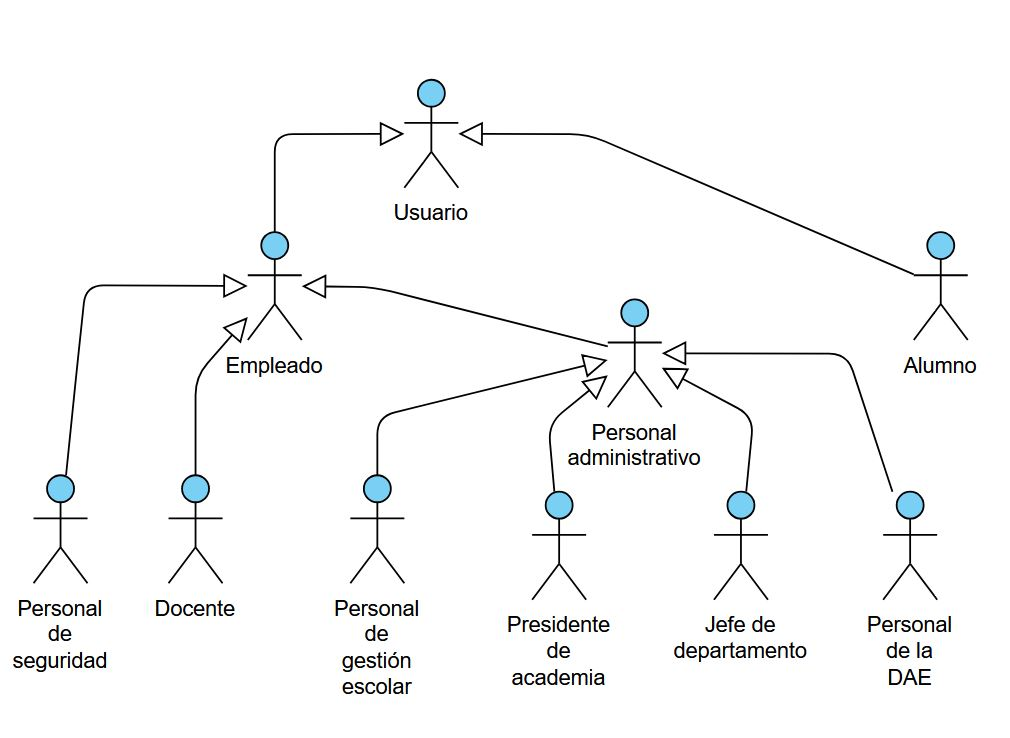
\includegraphics[width=.8\textwidth]{images/EstructuraU}}
		\caption{Estructura de los usuarios.}
		\label{fig:EstructuraU}
	\end{center}
\end{figure} 

En la figura \ref{fig:EstructuraU} se muestra la estructura de los usuarios y los tipos de usuario que están presentes en el sistema, en este se puede observar como todos los usuarios se derivan de un usuario general llamado usuario, posteriormente se divide en tipos; empleado y alumno. Después el empleado se subdivide dejando al personal de seguridad y al docente como empleados generales y creando un sub-usuario llamado personal administrativo el cual contiene al personal de gestión escolar, al presidente de academia, jefe de academia y al personal de la DAE. 

A continuación, se describirán las responsabilidades y los procesos de cada uno de los usuarios específicos (es decir los: los alumnos, personal de seguridad, docente, personal de gestión escolar, presidente de academia, jefe de departamento y personal de la DAE).

%\newpage



%\newpage

%\newpage



%---------------------------------------------------------
\section{Descripción de actores}

%---------------------------------------------------------
\begin{Usuario}{\hypertarget{tAlumno}{\subsection{Alumno}}}{
		Se refiere a las personas inscritas dentro de algún plan de estudios ofertado en la unidad académica.
	}
	\item[Responsabilidades:] \cdtEmpty
	\begin{itemize}
		\item Asistir puntualmente a las clases, prácticas y evaluaciones.
		\item Respetar a docentes, compañeros y personal administrativo.
		\item Cumplir con los requisitos y actividades de las asignaturas inscritas, incluyendo tareas, proyectos y exámenes.
		\item Realizar oportunamente los trámites escolares como inscripciones, reinscripciones, solicitudes de documentos oficiales, etc.
		\item Portar credencial institucional en todo momento.
	\end{itemize}
	

\end{Usuario}

\begin{Usuario}{\hypertarget{tPersonalSeguridad}{\subsection{Personal de seguridad}}}{
		Se refiere a las personas registradas como empleados y que permiten o no el acceso a la unidad académica.
	}
	\item[Responsabilidades:] \cdtEmpty
	\begin{itemize}
		\item Supervisar el acceso y la salida de alumnos, personal docente y visitantes, asegurándose de que cumplan con los protocolos establecidos.
		\item Verificar la identificación de las personas que ingresan a las instalaciones.
		\item Responder de manera oportuna a incidentes o emergencias dentro de las instalaciones.
		\item Brindar apoyo al personal, docentes o alumnos en caso de accidentes o situaciones de riesgo.
	\end{itemize}
	

\end{Usuario}

\begin{Usuario}{\hypertarget{tDocenteAplicador}{\subsection{Docente}}}{
		Se refiere a las personas registradas como empleados que dan clases a los alumnos y supervisan los ETS asignados.
	}
	\item[Responsabilidades:] \cdtEmpty
	\begin{itemize}
		\item Impartir las clases de manera clara, puntual y completa, cumpliendo con los objetivos de aprendizaje.
		\item Diseñar y aplicar instrumentos de evaluación justos, objetivos y alineados con los contenidos del curso.
		\item Orientar a los alumnos en el desarrollo de competencias y habilidades.
		\item Resolver dudas o problemáticas académicas dentro y fuera del aula, cuando sea necesario.
		\item Registrar la asistencia de los alumnos y reportar incidencias graves.
		\item Cumplir con la entrega de calificaciones y reportes en tiempo y forma.

	\end{itemize}
	

\end{Usuario}

\begin{Usuario}{\hypertarget{tPersonalGestion}{\subsection{Personal de gestión escolar}}}{
		Se refiere a las personas registradas como empleados y personal administrativo que realiza los procesos administrativos dentro de la ESCOM.
	}
	\item[Responsabilidades:] \cdtEmpty
	\begin{itemize}

		\item Gestionar el proceso de inscripción y reinscripción de los alumnos, verificando que cumplan con los requisitos establecidos.
		\item Mantener y actualizar el historial académico de los alumnos en los sistemas institucionales.
		\item Revisar y validar actas de nacimiento, certificados y otros documentos oficiales requeridos para el registro de los alumnos.
		\item Atender solicitudes y problemáticas relacionadas con registros, certificados, bajas temporales y procesos extraordinarios.
		\item Brindar orientación a alumnos y docentes sobre trámites escolares, fechas importantes y normatividad académica.
	\end{itemize}


\end{Usuario}

\begin{Usuario}{\hypertarget{tPersonalDAE}{\subsection{Personal de la DAE}}}{
		Se refiere a las personas registradas como empleados y personal administrativo que realiza los procesos administrativos dentro de la DAE.
	}
	\item[Responsabilidades:] \cdtEmpty
	\begin{itemize}

		\item Fomentar y coordinar actividades extracurriculares que complementen la formación académica, como talleres, conferencias, eventos culturales y deportivos.
		\item Supervisar programas de apoyo académico, como tutorías, orientación educativa y psicológica.
		\item Difundir información sobre programas de movilidad académica, intercambios, convenios nacionales e internacionales y programas de servicio social.
		\item Gestionar y emitir las credenciales oficiales del IPN para los alumnos.
		\item Verificar que los documentos requeridos para la emisión de la credencial estén completos y sean válidos.
		\item Coordinar el proceso de inscripción de los alumnos.
		\item Actualizar y mantener los registros académicos y administrativos de los alumnos. 
	\end{itemize}


\end{Usuario}

\begin{Usuario}{\hypertarget{tPresidente}{\subsection{Presidente de academia}}}{
	Se refiere a las personas registradas como empleados y personal administrativo que lidera la academia de una unidad académica o área de conocimiento dentro de la ESCOM.
	}
	\item[Responsabilidades:] \cdtEmpty
	\begin{itemize}

		\item Convocar y presidir las reuniones de academia, donde se toman decisiones sobre planes y programas de estudio.
		\item Coordinar la creación o actualización de planes y programas de estudio conforme a las necesidades del mercado laboral y las directrices institucionales.
		\item Verificar que los contenidos impartidos por los docentes sean consistentes con los objetivos de los programas.
		\item Detectar necesidades de capacitación entre los docentes y promover cursos o talleres. 
	\end{itemize}

\end{Usuario}

\begin{Usuario}{\hypertarget{tJefe}{\subsection{Jefe de departamento}}}{
	Se refiere a las personas registradas como empleados y personal administrativo que supervisa las actividades de una o más unidades académicas dentro de ESCOM.
}
\item[Responsabilidades:] \cdtEmpty
\begin{itemize}

	\item Administrar los recursos humanos y materiales asignados al departamento.
	\item Supervisar la implementación de los programas de estudio y el cumplimiento de los objetivos educativos.
	\item Promover y coordinar proyectos de investigación, desarrollo tecnológico o vinculación relacionados con el departamento.
	\item Atender quejas, sugerencias o problemas que surjan en el departamento, ya sea entre docentes o alumnos.
\end{itemize}

\end{Usuario}

A continuación se muestran los diagramas de casos de uso:

\begin{figure}[htbp!]
	\begin{center}
		\fbox{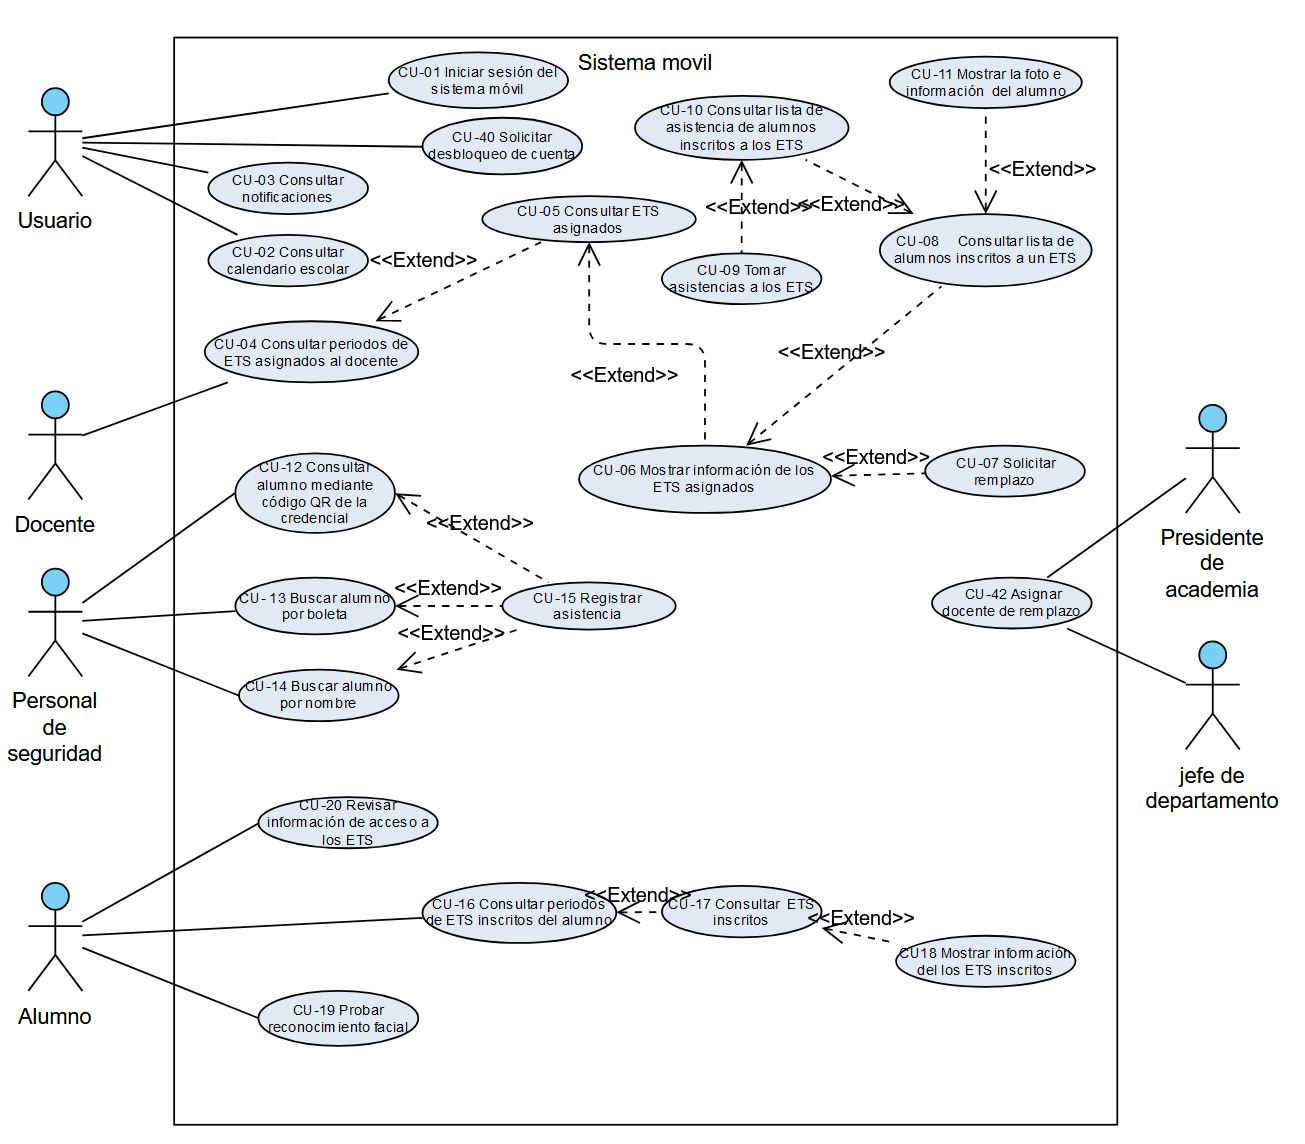
\includegraphics[width=.6\textwidth]{images/casosDeUso1}}
		\caption{Diagrama de casos de uso del sistema movil.}
		\label{fig:casosDeUso1}
	\end{center}
\end{figure}
En la figura \ref{fig:casosDeUso1} se muestra el diagrama de casos de uso del sistema móvil el cual es el sistema principal del trabajo terminal. En este diagrama se detalla la estructura del sistema, los casos de uso del docente, del alumno, del personal de seguridad, del presidente de academia y el jefe de departamento.
%\newpage
\begin{figure}[htbp!]
	\begin{center}
		\fbox{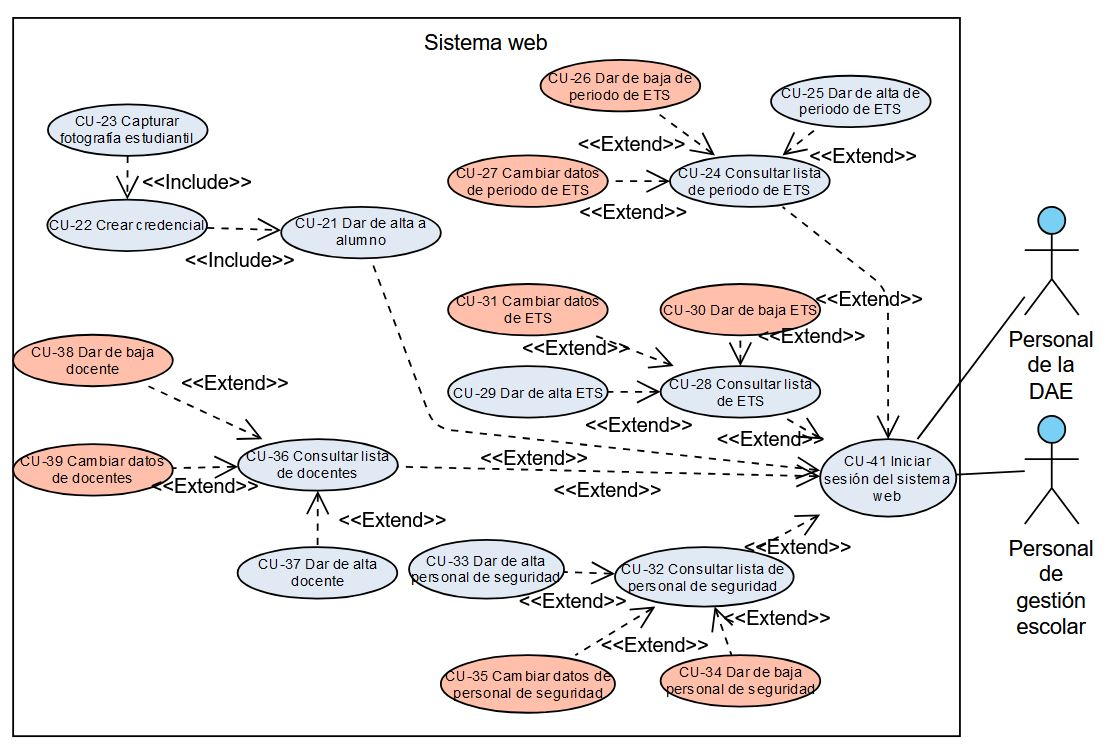
\includegraphics[width=.6\textwidth]{images/casosDeUso2}}
		\caption{Diagrama de casos de uso del sistema web.}
		\label{fig:casosDeUso2}
	\end{center}
\end{figure}

En la figura \ref{fig:casosDeUso2} se muestra el diagrama de casos de uso del sistema web el cual es el sistema secundario (la simulación de una parte del SAES y de la DAE) del trabajo terminal. En este diagrama se detalla la estructura del sistema, los casos de uso personal de la DAE y el personal de gestión escolar.

A continuación se detallan los casos de uso.

%---------------------------------------------------------
% CASOS DE USO

% !TeX root = ../ejemplo.tex

%--------------------------------------
\begin{UseCase}{CU01}{Iniciar sesión de personal escolar móvil}{
		Permitir que solo el personal escolar pueda acceder al sistema, además de separar completamente las funciones del alumno y el personal escolar.
	}
	\UCitem{Versión}{\color{Gray}1}
	\UCitem{Autor}{\color{Gray}Huertas Ramírez Daniel Martín}
	\UCitem{Supervisa}{\color{Gray}Ulises Vélez Saldaña.}
	\UCitem{Actor}{\hyperlink{Empleado}{Empleado} (\hyperlink{Docente}{Docente} y \hyperlink{Personal de seguridad}{Personal de seguridad})}
	\UCitem{Propósito}{Que el empelado pueda acceder al sistema móvil y sus funciones específicas. }
	\UCitem{Entradas}{\hyperlink{Empleado.RFC}{RFC}, \hyperlink{Empleado.Contraseña}{Contraseña}}
	\UCitem{Origen}{Teclado}
	\UCitem{Salidas}{Saludo del sistema, mención de su nombre.}
	\UCitem{Destino}{Pantalla \IUref{IUE01}{Pantalla Menú de docente} si es un docente o a la \IUref{IUE02}{Pantalla Menú del personal de seguridad} si es un personal de seguridad.}
	\UCitem{Precondiciones}{El empleado debe estar registrado en el sistema de la ESCOM.}
	\UCitem{Postcondiciones}{El empleado accede al sistema y podrá realizar las acciones pertinentes a su cargo.}
	\UCitem{Errores}{
		E1: Cuando falte algún dato requerido entonces el sistema muestra el mensaje {\bf MSG1-}{``Los campos no están correctamente llenados.''}
		
		E2: Cuando la cuenta esta bloqueada el sistema no deja entrar al empleado muestra el mensaje {\bf MSG2-}``Su cuenta esta bloqueada.''
		
		E3: Cuando la contraseña no corresponde al RFC ingresado el sistema no permite el acceso al empleado y se muestra el mensaje {\bf MSG3-} ``El RFC o la contraseña no corresponden con ningún empleado.''
		
		E4: Cuando se pierde la conexión durante el proceso, los procesos se cancelan y se muestra el mensaje {\bf MSG4-}  ``El proceso no se pudo realizar por un falló de red.''
		
		E5: Cuando se intenta iniciar varias veces sesión sin éxito la cuenta es bloqueada por seguridad y se muestra el mensaje {\bf MSG5-}  ``Su cuenta ha sido bloqueada por la gran cantidad de intentos de inicio sesión fallidos''.
	}
	\UCitem{Tipo}{Caso de uso primario}
	\UCitem{Observaciones}{}
\end{UseCase}
%--------------------------------------

\begin{UCtrayectoria}
	\UCpaso[\UCactor] Introduce su RFC y contraseña en el sistema vía la \IUref{IU01}{Pantalla de Iniciar sesión de personal escolar móvil}\label{CU01.introduceDatos}.
	\UCpaso[\UCactor] Confirma la operación presionando el botón \IUbutton{Entrar}.
	\UCpaso Verifica que todos los datos requeridos hayan sido capturados.
	\UCpaso Verifica que el empleado este registrado en el sistema.
	\UCpaso Verifica que la cuenta del empleado no este bloqueada.
	\UCpaso Verifica que la contraseña corresponda al RFC.
	\UCpaso Verifica que tipo acceso tiene este empleado.
	\UCpaso La sesión es iniciada con éxito.
	\UCpaso El Empleado es redirigido a la pantalla \IUref{IUE01}{Pantalla Menú de docente} si es un docente o a la pantalla \IUref{IUE02}{Menú de personal de seguridad} si es un personal de seguridad.
	
\end{UCtrayectoria}







\newpage

% !TeX root = ../ejemplo.tex

%--------------------------------------
\begin{UseCase}{CU-02}{Consultar calendario escolar}{
    Permitir que los usuarios vean el calendario escolar y puedan solicitar al sistema que les mencioné cuantos días faltan para que inicie el próximo periodo de ETS.
}
    \UCitem{Versión}{\color{Gray}1}
    \UCitem{Autor}{\color{Gray}Huertas Ramírez Daniel Martín}
    \UCitem{Supervisa}{\color{Gray}De la Cruz de la Cruz Alejandra.}
    \UCitem{Actor}{\hyperlink{Usuario}{Usuario}}
    \UCitem{Propósito}{Que el usuario consulte cuantos días faltan para el próximo periodo de ETS.}
    \UCitem{Entradas}{Ninguna}
    \UCitem{Origen}{Pantalla táctil}
    \UCitem{Salidas}{Menciona cuantos días faltan para el periodo de ETS o si menciona que ya es periodo de ETS.}
    \UCitem{Destino}{Ninguno}
    \UCitem{Precondiciones}{El usuario debe de haber iniciado sesión.}
    \UCitem{Postcondiciones}{El usuario recibe información sobre la fecha del periodo de ETS actual.}
    \UCitem{Errores}{
        E1: Cuando es periodo de ETS el sistema muestra el mensaje {\bf MSG-6}{``Actualmente es periodo de ETS.''}

        E2: Cuando no se ha establecido un periodo de ETS actual, el sistema muestra el mensaje {\bf MSG-7}{``Actualmente el periodo de ETS no ha sido establecido.''}
    
    }
    \UCitem{Tipo}{Caso de uso primario}
    \UCitem{Observaciones}{Ninguna}
\end{UseCase}
%-------------------------------------- 

\begin{UCtrayectoria}
    \UCpaso[\UCactor] El usuario accede a la pantalla \IUref{IU02}{Pantalla Consultar calendario escolar}\label{CU02.introduceDatos} para la app móvil y \IUref{IU02-2}{Pantalla Consultar calendario escolar} para el sistema web mediante el botón con forma de calendario en cualquier pantalla excepto el inicio de sesión.
    \UCpaso[\UCactor] El usuario decide consultar cuantos días faltan para que el periodo de ETS inicie oprimiendo el botón\IUbutton{Calcular cuantos días faltan para el periodo de ETS}.
    \UCpaso El sistema calcula cuantos días faltan tomando el día actual y el día de inicio del periodo de ETS.
    \UCpaso El sistema regresa cuantos días faltan para que el periodo de ETS inicie.
    \UCpaso [\UCactor] El usuario verifica cuantos días faltan para que inicie el periodo de ETS.
\end{UCtrayectoria}








\newpage

% !TeX root = ../ejemplo.tex

%--------------------------------------
\begin{UseCase}{CU-03}{Consultar notificaciones}{
    Permitir a los usuarios revisar sus notificaciones con más detenimiento y establecerlas como leídas.
}
    \UCitem{Versión}{\color{Gray}1}
    \UCitem{Autor}{\color{Gray}Huertas Ramírez Daniel Martín}
    \UCitem{Supervisa}{\color{Gray}De la Cruz de la Cruz Alejandra.}
    \UCitem{Actor}{\hyperlink{Usuario}{Usuario}}
    \UCitem{Propósito}{Que el usuario revise sus notificaciones con detenimiento y las establezca como leídas.}
    \UCitem{Entradas}{Ninguna}
    \UCitem{Origen}{Pantalla táctil}
    \UCitem{Salidas}{Menciona que la notificación seleccionada ha sido establecida como leída.}
    \UCitem{Destino}{Ninguno}
    \UCitem{Precondiciones}{El usuario debe de haber iniciado sesión.}
    \UCitem{Postcondiciones}{El usuario revisó sus notificaciones.}
    \UCitem{Errores}{
        E1: Cuando el usuario no tiene notificaciones el sistema muestra el mensaje {\bf MSG-8}{``Actualmente no hay notificaciones.''}    
    }
    \UCitem{Tipo}{Caso de uso primario}
    \UCitem{Observaciones}{}

\end{UseCase}
%-------------------------------------- 

\begin{UCtrayectoria}
    \UCpaso[\UCactor] El usuario accede a la pantalla \IUref{IU03}{Pantalla Consultar notificaciones}\label{CU03.introduceDatos} para la app móvil  mediante el botón con forma de campana en cualquier pantalla excepto los inicios de sesión.
    \UCpaso[\UCactor] El usuario decide consultar sus notificaciones más actuales \Trayref{A}.
    \UCpaso[\UCactor] El usuario marco como leídas las notificaciones que acaba de leer mediante el botón con forma de palomita especifico de cada notificación.
    \UCpaso El sistema marca como leídas las notificaciones.

\end{UCtrayectoria}

\begin{UCtrayectoriaA}{A}{El usuario quiere consultar las notificaciones de una fecha específica}
	\UCpaso[\UCactor] El usuario usa el buscador de la parte superior para buscar notificaciones según su fecha.
	\UCpaso[\UCactor] El usuario marco como leídas las notificaciones que acaba de leer mediante el botón con forma de palomita especifico de cada notificación.
	\UCpaso El sistema marca como leídas las notificaciones.

\end{UCtrayectoriaA}



\newpage

% \IUref{IUAdmPS}{Administrar Planta de Selección}
% \IUref{IUModPS}{Modificar Planta de Selección}
% \IUref{IUEliPS}{Eliminar Planta de Selección}

%-------------------------------------- COMIENZA descripción del caso de uso.

%\begin{UseCase}[archivo de imágen]{UCX}{Nombre del Caso de uso}{
%--------------------------------------
\begin{UseCase}{CU-04}{Consultar periodos de ETS asignados al docente}{
		Este caso de uso permite al docente consultar los periodos de ETS que tiene asignados. 
	}
	\UCitem{Versión}{\color{Gray}1.0}
	\UCitem{Autor}{\color{Gray}De la cruz De la cruz Alejandra}
	\UCitem{Supervisa}{\color{Gray}Ulises Velez Saldaña}
	\UCitem{Actor}{\hyperlink{Docente}{Docente}}
	\UCitem{Propósito}{Permitir al docente consultar los periodos de ETS que le han sido asignados.}
	\UCitem{Entradas}{Ninguna}
	\UCitem{Origen}{Pantalla táctil}
	\UCitem{Salidas}{Lista de periodos de ETS asignados.}
	\UCitem{Destino}{\IUref{IU04}{Pantalla Periodo de ETS}}
	\UCitem{Precondiciones}{El docente debe estar autenticado en el sistema.}
	\UCitem{Postcondiciones}{El docente ha consultado los periodos de ETS asignados.}
	\UCitem{Errores}{
			E1:El sistema no puede recuperar la información de los periodos.
			
			E2: No hay periodos de ETS asignados al docente. }
	\UCitem{Tipo}{Se extiende del CU}
	\UCitem{Observaciones}{Ninguna}
\end{UseCase}
%--------------------------------------
\begin{UCtrayectoria}
	\UCpaso[\UCactor] Accede a la \IUref{IUE01}{Pantalla Menú del docente} después de haber iniciado sesión.
	\UCpaso[\UCactor] Presiona el botón \IUbutton{Consultar periodos de ETS}.
	\UCpaso Verifica que el docente cuente con periodos de ETS. \Trayref{A}.
	\UCpaso Busca en la base de datos los periodos de ETS asignados al docente.
	\UCpaso Despliega la lista de periodos de ETS asignados al docente en la \IUref{IU04}{Pantalla Periodo de ETS}.
\end{UCtrayectoria}
%--------------------------------------        
\begin{UCtrayectoriaA}{A}{No hay periodos asignados al docente}
	\UCpaso Verifica y no encuentra registros de periodos de ETS asignados al docente.
	\UCpaso Muestra un mensaje: {\bf MSG10-}{``No hay periodos de ETS asignados.''}
	\UCpaso[\UCactor] Presiona el botón \IUbutton{Regresar} para volver a la pantalla anterior.
	\UCpaso Fin de la trayectoria alternativa.
\end{UCtrayectoriaA}
%--------------------------------------        
\begin{UCtrayectoriaA}{B}{Error en la conexión con la base de datos}
	\UCpaso Muestra un mensaje de error: {\bf MSG11-}{``Error al consultar la base de datos. Intente nuevamente más tarde.''}
	\UCpaso[\UCactor] Presiona el botón \IUbutton{Aceptar} para cerrar el mensaje.
	\UCpaso[\UCactor] Puede intentar la consulta nuevamente o presionar el botón \IUbutton{Regresar} para volver a la pantalla anterior.
	\UCpaso Fin de la trayectoria alternativa.
\end{UCtrayectoriaA}
%-------------------------------------- TERMINA descripción del caso de uso.

\newpage

% \IUref{IUAdmPS}{Administrar Planta de Selección}
% \IUref{IUModPS}{Modificar Planta de Selección}
% \IUref{IUEliPS}{Eliminar Planta de Selección}

%-------------------------------------- COMIENZA descripción del caso de uso.

%\begin{UseCase}[archivo de imágen]{UCX}{Nombre del Caso de uso}{
%--------------------------------------
\begin{UseCase}{CU-05}{Consultar ETS asignados}{
		Este caso de uso permite al docente consultar los ETS que tiene asignados.
	}
	\UCitem{Versión}{\color{Gray}1.0}
	\UCitem{Autor}{\color{Gray}De la cruz De la cruz Alejandra}
	\UCitem{Supervisa}{\color{Gray}Ulises Velez Saldaña}
	\UCitem{Actor}{\hyperlink{Docente}{Docente}}
	\UCitem{Propósito}{Permitir al docente consultar los ETS que le han sido asignados.}
	\UCitem{Entradas}{Selecciona un periodo}
	\UCitem{Origen}{Pantalla táctil}
	\UCitem{Salidas}{Lista de ETS asignados.}
	\UCitem{Destino}{\IUref{IU05}{Pantalla de Consultar ETS}}
	\UCitem{Precondiciones}{El docente debe estar autenticado en el sistema.}
	\UCitem{Postcondiciones}{El docente ha consultado los ETS asignados.}
	\UCitem{Errores}{
			E1: El sistema no puede recuperar la información de los ETS asignados.
			
			E2: No hay ETS asignados al docente.}
	\UCitem{Tipo}{Se extiende del CU01 Iniciar Sesión del docente}
	\UCitem{Observaciones}{Ninguna}
\end{UseCase}
%--------------------------------------
\begin{UCtrayectoria}
	\UCpaso[\UCactor] Selecciona el período académico que desea consultar desde la \IUref{IU04}{Pantalla Periodo de ETS}.
	\UCpaso Verifica que el docente tenga ETS asignados en el periodo seleccionado \Trayref{A}.
	\UCpaso Despliega la lista de ETS asignados al docente en la \IUref{IU05}{Pantalla de Consultar ETS}.
\end{UCtrayectoria}

%--------------------------------------        
\begin{UCtrayectoriaA}{A}{No hay ETS asignados en el periodo seleccionado}
	\UCpaso Muestra un mensaje: {\bf MSG-12-}{``No hay ETS asignados actualmente.''}
	\UCpaso[\UCactor] Presiona el botón \IUbutton{Regresar} para volver a la pantalla anterior.
	\UCpaso Fin de la trayectoria alternativa.
\end{UCtrayectoriaA}
%--------------------------------------        
\begin{UCtrayectoriaA}{B}{Error en la conexión con la base de datos}
	\UCpaso Muestra un mensaje de error: {\bf MSG11-}{``Error al consultar la base de datos. Intente nuevamente más tarde.''}
	\UCpaso[\UCactor] Presiona el botón \IUbutton{Aceptar} para cerrar el mensaje.
	\UCpaso[\UCactor] Puede intentar la consulta nuevamente o presionar el botón \IUbutton{Regresar} para volver a la pantalla anterior.
	\UCpaso Fin de la trayectoria alternativa.
\end{UCtrayectoriaA}

%-------------------------------------- TERMINA descripción del caso de uso.
\newpage

% \IUref{IUAdmPS}{Administrar Planta de Selección}
% \IUref{IUModPS}{Modificar Planta de Selección}
% \IUref{IUEliPS}{Eliminar Planta de Selección}

%-------------------------------------- COMIENZA descripción del caso de uso.

%\begin{UseCase}[archivo de imágen]{UCX}{Nombre del Caso de uso}{
%--------------------------------------
% !TeX root = ../ejemplo.tex
\begin{UseCase}{CU-06}{Mostrar información de los ETS asignados}{
	Este caso de uso permite al docente visualizar la información detallada de los ETS que tiene asignados.
}
\UCitem{Versión}{\color{Gray}1.0}
\UCitem{Autor}{\color{Gray}De la cruz De la cruz Alejandra}
\UCitem{Supervisa}{\color{Gray}Huertas Ramírez Daniel Martín}
\UCitem{Actor}{\hyperlink{PersonalAcademico}{Docente}}
\UCitem{Propósito}{Permite al docente visualizar la información detallada de cada ETS que tiene asignado.}
\UCitem{Entradas}{Ninguna}
\UCitem{Origen}{Pantalla táctil}
\UCitem{Salidas}{Detalle de ETS asignado.}
\UCitem{Destino}{\IUref{IU06}{Pantalla Información de ETS}}
\UCitem{Precondiciones}{El docente debe estar autenticado y tener ETS asignados en el sistema.}
\UCitem{Postcondiciones}{El docente ha visualizado la información detallada de sus ETS asignados.}
\UCitem{Errores}{
		E1: El sistema no puede recuperar la información detallada de los ETS y muestra el mensaje {\bf MSG-12}{``Información no disponible para el ETS seleccionado''}.
		E2: Error en la conexión con la base de datos y muestra el mensaje y muestra el mensaje {\bf MSG-9}{``Error al consultar la base de datos. Intente nuevamente más tarde.''}.
}
\UCitem{Tipo}{Se entiende del CU-05 Mostrar información de los ETS asignados}
\UCitem{Observaciones}{Ninguna}
\end{UseCase}
%--------------------------------------
\begin{UCtrayectoria}
\UCpaso[\UCactor] El docente selecciona el ETS que desea visualizar desde la \IUref{IU05}{Pantalla  Consultar ETS}.
\UCpaso[\UCsist] El sistema verifica si existen detalles disponibles para el ETS seleccionado. \Trayref{A}
\UCpaso El sistema despliega la información detallada de cada ETS asignado en la \IUref{IU06}{Pantalla Información de ETS}
\end{UCtrayectoria}
%--------------------------------------        
\begin{UCtrayectoriaA}{A}{No hay detalles disponibles para el ETS seleccionado}
\UCpaso El sistema muestra un mensaje: {\bf MSG-12}{``Información no disponible para el ETS seleccinado''}
\UCpaso[\UCactor] El docente presiona el botón \IUbutton{Regresar} para volver a la lista de ETS.
\UCpaso Fin de la trayectoria alternativa.
\end{UCtrayectoriaA}

%--------------------------------------        
\begin{UCtrayectoriaA}{B}{Error en la conexión con la base de datos}
\UCpaso El sistema muestra un mensaje de error: {\bf MSG-9}{``Error al consultar la base de datos. Intente nuevamente más tarde.''}
\UCpaso[\UCactor] El docente presiona el botón \IUbutton{Aceptar} para cerrar el mensaje.
\UCpaso[\UCactor] El docente puede intentar la consulta nuevamente o presionar el botón \IUbutton{Regresar} para volver a la pantalla anterior.
\UCpaso Fin de la trayectoria alternativa.
\end{UCtrayectoriaA}

%-------------------------------------- TERMINA descripción del caso de uso.


\newpage

% \IUref{IUAdmPS}{Administrar Planta de Selección}
% \IUref{IUModPS}{Modificar Planta de Selección}
% \IUref{IUEliPS}{Eliminar Planta de Selección}

%-------------------------------------- COMIENZA descripción del caso de uso.

%\begin{UseCase}[archivo de imágen]{UCX}{Nombre del Caso de uso}{
%--------------------------------------
\begin{UseCase}{CU-07}{Asignar docente ayudante}{
		Este caso de uso permite a un docente solicitar la asignación de un docente ayudante para aplicar el ETS en su lugar en caso de no poder asistir.
	}
	\UCitem{Versión}{\color{Gray}1.0}
	\UCitem{Autor}{\color{Gray}De la cruz De la cruz Alejandra}
	\UCitem{Supervisa}{\color{Gray}Ulises Velez Saldaña}
	\UCitem{Actor}{\hyperlink{Docente}{Docente}}
	\UCitem{Propósito}{Permitir al docente asignado para un ETS solicitar ayuda de otro docente para realizar la aplicación en su lugar.}
	\UCitem{Entradas}{
		\begin{itemize}
			\item Identificador del ETS.
			\item Identificador del docente ayudante solicitado.
		\end{itemize}
	}
	\UCitem{Origen}{Teclado}
	\UCitem{Salidas}{Confirmación de la asignación del docente ayudante.}
	\UCitem{Destino}{{\bf MSG-14-}{``El docente ayudante ha sido asignado exitosamente para la aplicación del ETS.''}}
	\UCitem{Precondiciones}{El docente debe estar autenticado en el sistema y tener un ETS asignado.}
	\UCitem{Postcondiciones}{El docente ayudante ha sido asignado al ETS en lugar del docente asignado.}
	\UCitem{Errores}{
			E1: El sistema pierde la conexión al intentar registrar la asignación.
	}
	\UCitem{Tipo}{Se extiende del CU}
	\UCitem{Observaciones}{Ninguna}
\end{UseCase}
%--------------------------------------
\begin{UCtrayectoria}
	\UCpaso[\UCactor] El docente accede a la \IUref{IU06}{Pantalla Información de ETS}.
	\UCpaso[\UCactor] Selecciona la opción \IUbutton{Solicitar docente ayudante} para el ETS asignado.
	\UCpaso Ingresa el identificador del docente ayudante.
	\UCpaso El sistema verifica la existencia del ETS. \Trayref{A}
	\UCpaso El sistema verifica la disponibilidad del docente ayudante para la fecha del ETS. \Trayref{B} \Trayref{D}
	\UCpaso El sistema registra la asignación del docente ayudante en la base de datos. \Trayref{C}
	\UCpaso Muestra un mensaje de confirmación: {\bf MSG-14-}{``El docente ayudante ha sido asignado exitosamente para la aplicación del ETS.''}
\end{UCtrayectoria}
%--------------------------------------        
\begin{UCtrayectoriaA}{A}{El ETS no existe o ya ha sido aplicado}
	\UCpaso[\UCactor] El sistema muestra un mensaje: {\bf MSG-15-}{``El ETS especificado no existe o ya ha sido aplicado. Verifique la información e intente nuevamente.''}
	\UCpaso[\UCactor] El docente puede reingresar el identificador del ETS o regresar a la pantalla anterior.
	\UCpaso Fin de la trayectoria alternativa.
\end{UCtrayectoriaA}
%--------------------------------------        
\begin{UCtrayectoriaA}{B}{Docente ayudante no disponible en la fecha}
	\UCpaso El sistema detecta que el docente ayudante solicitado no está disponible para la fecha del ETS.
	\UCpaso[\UCactor] El sistema muestra un mensaje: {\bf MSG-16-}{``El docente ayudante no está disponible en la fecha especificada.''}
	\UCpaso[\UCactor] El docente puede seleccionar otro docente o intentar una nueva asignación.
	\UCpaso Fin de la trayectoria alternativa.
\end{UCtrayectoriaA}
%--------------------------------------        
\begin{UCtrayectoriaA}{C}{Error al registrar la asignación}
	\UCpaso Ocurrió un error al intentar registrar la asignación en la base de datos debido a una pérdida de conexión.
	\UCpaso[\UCactor] El sistema muestra un mensaje de error:  {\bf MSG-4} {``El proceso no se pudo realizar por un falló de red.''}
	\UCpaso[\UCactor] El docente presiona \IUbutton{Aceptar} y puede intentar la asignación nuevamente más tarde.
	\UCpaso Fin de la trayectoria alternativa.
\end{UCtrayectoriaA}
%--------------------------------------
\begin{UCtrayectoriaA}{D}{Docente ayudante ya asignado en otro ETS}
	\UCpaso El sistema detecta que el docente solicitado ya está asignado como ayudante en otro ETS en la misma fecha y horario.
	\UCpaso[\UCactor] El sistema muestra un mensaje: {\bf MSG-17-}{``El docente ya está asignado en otro ETS en el mismo horario.''}
	\UCpaso[\UCactor] El docente solicitante puede elegir otro docente o ajustar la fecha de solicitud.
	\UCpaso Fin de la trayectoria alternativa.
\end{UCtrayectoriaA}

%-------------------------------------- TERMINA descripción del caso de uso.
\newpage

% \IUref{IUAdmPS}{Administrar Planta de Selección}
% \IUref{IUModPS}{Modificar Planta de Selección}
% \IUref{IUEliPS}{Eliminar Planta de Selección}

%-------------------------------------- COMIENZA descripción del caso de uso.

%\begin{UseCase}[archivo de imágen]{UCX}{Nombre del Caso de uso}{
%--------------------------------------
\begin{UseCase}{CU-08}{Consultar lista de alumnos inscritos a un ETS}{
		Este caso de uso permite al docente consultar la lista de los alumnos inscritos a un ETS asignado.
	}
	\UCitem{Versión}{\color{Gray}1.0}
	\UCitem{Autor}{\color{Gray}De la cruz De la cruz Alejandra}
	\UCitem{Supervisa}{\color{Gray}Huertas Ramírez Daniel Martín}
	\UCitem{Actor}{\hyperlink{PersonalAcademico}{Docente}}
	\UCitem{Propósito}{Permitir al docente visualizar la lista de alumnos inscritos en un ETS para verificar su asistencia.}
	\UCitem{Entradas}{Ninguna}
	\UCitem{Origen}{Pantalla táctil}
	\UCitem{Salidas}{Lista de los alumnos inscritos al ETS.}
	\UCitem{Destino}{\IUref{IU13}{Pantalla consultar lista de alumnos inscritos a un ETS}.}
	\UCitem{Precondiciones}{El docente debe estar autenticado y tener asignado el ETS correspondiente.}
	\UCitem{Postcondiciones}{El docente ha visualizado la lista de asistencia de los alumnos inscritos al ETS.}
	\UCitem{Errores}{
			E1: El ETS seleccionado no tiene alumnos inscritos y se muestra el mensaje {\bf MSG-14}{``No hay alumnos inscritos en este ETS.''}.
			
			E2: El sistema pierde la conexión al intentar recuperar la lista de asistencia y se muestra el mensaje {\bf MSG-9}{``Error al consultar la base de datos. Intente nuevamente más tarde.''}.
	}
	\UCitem{Tipo}{Se entiende del CU06 Mostrar información de los ETS asignados}
	\UCitem{Observaciones}{Ninguna}
\end{UseCase}
%--------------------------------------
\begin{UCtrayectoria}
	\UCpaso[\UCactor] El docente presiona el botón \IUbutton{Ver alumnos} desde la pantalla \IUref{IU06}{Pantalla de Información de ETS}.
	\UCpaso El sistema verifica la existencia del ETS y que tenga alumnos inscritos. \Trayref{A}.
	\UCpaso El sistema recupera la lista de alumnos inscritos en el ETS. \Trayref{B}
	\UCpaso El sistema muestra la lista de alumnos inscritos en la \IUref{IU13}{Pantalla consultar lista de alumnos inscritos a un ETS}.
\end{UCtrayectoria}

%--------------------------------------        
\begin{UCtrayectoriaA}{A}{El ETS no tiene alumnos inscritos}
	\UCpaso El sistema muestra un mensaje: {\bf MSG-14}{``No hay alumnos inscritos en este ETS.''}
	\UCpaso[\UCactor] El docente presiona el botón \IUbutton{Regresar} para volver a la pantalla anterior donde se muestra la información detallada del ETS.
	\UCpaso Fin de la trayectoria alternativa.
\end{UCtrayectoriaA}
%--------------------------------------        
\begin{UCtrayectoriaA}{B}{Error en la conexión con la base de datos}
	\UCpaso El sistema muestra un mensaje de error: {\bf MSG-9}{``Error al consultar la base de datos. Intente nuevamente más tarde.''}
	\UCpaso[\UCactor] El docente presiona el botón \IUbutton{Aceptar} para cerrar el mensaje.
	\UCpaso[\UCactor] El docente puede intentar la consulta nuevamente.
	\UCpaso Fin de la trayectoria alternativa.
\end{UCtrayectoriaA}
%-------------------------------------- TERMINA descripción del caso de uso.

\newpage

% \IUref{IUAdmPS}{Administrar Planta de Selección}
% \IUref{IUModPS}{Modificar Planta de Selección}
% \IUref{IUEliPS}{Eliminar Planta de Selección}

%-------------------------------------- COMIENZA descripción del caso de uso.

%\begin{UseCase}[archivo de imágen]{UCX}{Nombre del Caso de uso}{
%--------------------------------------
\begin{UseCase}{CU-09}{Tomar asistencias a los ETS}{
		Este caso de uso permite al docente registrar la asistencia de los alumnos inscritos a un ETS asignado.
	}
	\UCitem{Versión}{\color{Gray}1.0}
	\UCitem{Autor}{\color{Gray}De la cruz De la cruz Alejandra}
	\UCitem{Supervisa}{\color{Gray}Huertas Ramírez Daniel Martín}
	\UCitem{Actor}{\hyperlink{Docente}{Docente}}
	\UCitem{Propósito}{Permitir al docente registrar la asistencia de los alumnos que estén inscritos a un ETS.}
	\UCitem{Entradas}{-}
	\UCitem{Origen}{Pantalla táctil}
	\UCitem{Salidas}{Confirmación del registro de asistencia de los alumnos.}
	\UCitem{Destino}{\IUref{IU08}{Lista de asistencia de ETS.}}
	\UCitem{Precondiciones}{El docente debe estar autenticado y asignado al ETS correspondiente.}
	\UCitem{Postcondiciones}{La asistencia de los alumnos ha sido registrada en el sistema para el ETS.}
	\UCitem{Errores}{
		\begin{itemize}
			\item El ETS seleccionado no tiene alumnos inscritos y se muestra el mensaje {\bf MSG-16}{``No hay alumnos inscritos en este ETS.''}
			\item El sistema pierde la conexión al intentar registrar la asistencia y se muestra el mensaje {\bf MSG-9}{``Error al consultar la base de datos. Intente nuevamente más tarde.''}
			\item El sistema no logro activar la camara y se muestra el mensaje {\bf MSG-17}{``No se pudo activar la cámara o reconocer la identidad. Intente nuevamente.''}
		\end{itemize}
	}
	\UCitem{Tipo}{Se entiende del CU-10 Consultar lista de asistencia de alumnos inscritos a los ETS}
	\UCitem{Observaciones}{}
\end{UseCase}
%--------------------------------------
\begin{UCtrayectoria}
	\UCpaso[\UCactor] El docente presiona el recuadro con la información del alumno que desee desde la pantalla \IUref{IU08}{Lista de asistencia de ETS}.
	\UCpaso El sistema le muestra una imagen del alumno al docente.
	\UCpaso[\UCactor] El docente no esta seguro de la identidad del alumno, por lo que decide usar el reconocimiento facial, accediendo a la pantalla \IUref{IU17}{Pantalla Reconocimiento facial} presionando el texto de \IUbutton{Estatus}. \Trayref{A} \Trayref{B}
	\UCpaso El sistema activa la cámara y comienza el proceso de reconocimiento facial de los alumnos presentes \IUref{IU17}{Pantalla Reconocimiento facial}. \Trayref{C} \Trayref{D}
	\UCpaso El sistema analiza la imagen de cada alumno y muestra un indicador:
	\begin{itemize}
		\item Verde: El sistema está casi seguro de que la persona es quien dice ser y muestra las características coincidentes.
		\item Amarillo: El sistema no está seguro y necesita la ayuda del docente para confirmar la identidad, mostrando tanto las características coincidentes como las que no coinciden. \Trayref{E}
		\item Rojo: El sistema está casi seguro de que la persona no es quien dice ser y muestra las características que no coinciden. \Trayref{F}
	\end{itemize}
	\UCpaso[\UCactor] El docente revisa las características del alumno y decide si confirma la identidad del alumno cuando el indicador marque el color Amarillo. 
	\UCpaso El sistema marca la asistencia de cada alumno.
	\UCpaso[\UCactor] El docente confirma el registro de asistencia.
	\UCpaso El sistema guarda la asistencia y muestra un mensaje de confirmación: {\bf MSG-15}{``Asistencia registrada exitosamente.''}
	\UCpaso El sistema muestra la lista de asistencia de los alumnos en la \IUref{IU08}{Pantalla Lista de asistencia de ETS.}
\end{UCtrayectoria}
%--------------------------------------        
\begin{UCtrayectoriaA}{A}{El Docente está seguro de la identidad del alumno sin la necesidad de usar el reconocimiento facial y decide que le registrara asistencia sin la necesidad del reconocimiento facial}
	\UCpaso[\UCactor] El docente presiona el botón \IUbutton{Registrar asistencia}.
	\UCpaso El sistema actualiza la asistencia.
	\UCpaso Fin de la trayectoria alternativa.
\end{UCtrayectoriaA}
%--------------------------------------        
\begin{UCtrayectoriaA}{B}{El Docente no está seguro de la identidad del alumno sin la necesidad de usar el reconocimiento facial y decide que no le registrara asistencia}
	\UCpaso[\UCactor] El docente presiona el botón \IUbutton{No registrar asistencia}.
	\UCpaso El sistema no actualiza la asistencia.
	\UCpaso Fin de la trayectoria alternativa.
\end{UCtrayectoriaA}        
%--------------------------------------        
\begin{UCtrayectoriaA}{C}{El ETS no tiene alumnos inscritos}
	\UCpaso El sistema muestra un mensaje: {\bf MSG-16}{``No hay alumnos inscritos en este ETS.''}
	\UCpaso[\UCactor] El docente presiona el botón \IUbutton{Regresar} para volver a la pantalla anterior.
	\UCpaso Fin de la trayectoria alternativa.
\end{UCtrayectoriaA}
%--------------------------------------        
\begin{UCtrayectoriaA}{D}{Error en la conexión con la base de datos}
	\UCpaso El sistema muestra un mensaje de error: {\bf MSG-9}{``Error al consultar la base de datos. Intente nuevamente más tarde.''}
	\UCpaso[\UCactor] El docente presiona el botón \IUbutton{Aceptar} para cerrar el mensaje.
	\UCpaso[\UCactor] El docente puede intentar registrar la asistencia.
	\UCpaso Fin de la trayectoria alternativa.
\end{UCtrayectoriaA}
%--------------------------------------        
\begin{UCtrayectoriaA}{E}{El sistema detecta incertidumbre en la identidad de un alumno}
	\UCpaso El sistema detecta las características coincidentes como las que no coinciden con el alumno.
	\UCpaso[\UCactor] El docente revisa la información proporcionada y toma una decisión sobre la identidad del alumno.
	\UCpaso[\UCactor] El docente confirma o corrige la asistencia.
	\UCpaso El sistema actualiza la asistencia según la confirmación del docente.
	\UCpaso El sistema muestra la lista de asistencia de los alumnos actualizada en la \IUref{IU08}{Pantalla Lista de asistencia de ETS}.
	\UCpaso Fin de la trayectoria alternativa.
\end{UCtrayectoriaA}
%--------------------------------------        
\begin{UCtrayectoriaA}{F}{El sistema identifica que el alumno no coincide con la foto registrada}
	\UCpaso El sistema muestra al docente las características que no coinciden.
	\UCpaso[\UCactor] El docente revisa las discrepancias y decide marcar al alumno como ausente o realizar una verificación adicional.
	\UCpaso El sistema actualiza la asistencia.
	\UCpaso El sistema muestra la lista de asistencia de los alumnos actualizada en la \IUref{IU08}{Pantalla Lista de asistencia de ETS}.
	\UCpaso Fin de la trayectoria alternativa.
\end{UCtrayectoriaA}

%-------------------------------------- TERMINA descripción del caso de uso.
\newpage

% \IUref{IUAdmPS}{Administrar Planta de Selección}
% \IUref{IUModPS}{Modificar Planta de Selección}
% \IUref{IUEliPS}{Eliminar Planta de Selección}

%-------------------------------------- COMIENZA descripción del caso de uso.

%\begin{UseCase}[archivo de imágen]{UCX}{Nombre del Caso de uso}{
%--------------------------------------
\begin{UseCase}{CU-10}{Consultar lista de asistencia de alumnos inscritos a los ETS}{
		Este caso de uso permite al docente visualizar la asistencia de los alumnos inscritos a un ETS asignado.
	}
	\UCitem{Versión}{\color{Gray}1.0}
	\UCitem{Autor}{\color{Gray}De la cruz De la cruz Alejandra}
	\UCitem{Supervisa}{\color{Gray}Huertas Ramírez Daniel Martin}
	\UCitem{Actor}{\hyperlink{Docente}{Docente}}
	\UCitem{Propósito}{Permitir al docente registrar la asistencia de los alumnos que estén inscritos a un ETS.}
	\UCitem{Entradas}{Ninguna}
	\UCitem{Origen}{Pantalla táctil}
	\UCitem{Salidas}{Confirmación del registro de asistencia de los alumnos.}
	\UCitem{Destino}{\IUref{IU08}{Lista de asistencia de ETS.}}
	\UCitem{Precondiciones}{El docente debe estar autenticado y asignado al ETS correspondiente.}
	\UCitem{Postcondiciones}{La asistencia de los alumnos ha sido registrada en el sistema para el ETS.}
	\UCitem{Errores}{
		\begin{itemize}
			\item El ETS seleccionado no tiene alumnos inscritos y se muestra el mensaje {\bf MSG-16}{``No hay alumnos inscritos en este ETS.''}
			\item El sistema pierde la conexión al intentar registrar la asistencia y se muestra el mensaje {\bf MSG-9}{``Error al consultar la base de datos. Intente nuevamente más tarde.''}
		\end{itemize}
	}
	\UCitem{Tipo}{Se entiende del CU-10 consultar lista de asistencia de alumnos inscritos a los ETS}
	\UCitem{Observaciones}{}
\end{UseCase}
%--------------------------------------
\begin{UCtrayectoria}
	\UCpaso[\UCactor] El docente presiona el botón \IUbutton{Tomar asistencia} desde la pantalla \IUref{IU13}{Pantalla Lista de alumno}.
	\UCpaso El sistema activa la cámara y comienza el proceso de reconocimiento facial de los alumnos presentes. \Trayref{A} \Trayref{B}
	\UCpaso El sistema analiza la imagen de cada alumno y muestra un indicador:
	\begin{itemize}
		\item Verde: El sistema está casi seguro de que la persona es quien dice ser y muestra las características coincidentes.
		\item Amarillo: El sistema no está seguro y necesita la ayuda del docente para confirmar la identidad, mostrando tanto las características coincidentes como las que no coinciden. \Trayref{C}
		\item Rojo: El sistema está casi seguro de que la persona no es quien dice ser y muestra las características que no coinciden. \Trayref{D}
	\end{itemize}
	\UCpaso[\UCactor] El docente revisa las características del alumno y decide si confirma la identidad del alumno cuando el indicador marque el color Amarillo. 
	\UCpaso El sistema marca la asistencia de cada alumno.
	\UCpaso[\UCactor] El docente confirma el registro de asistencia.
	\UCpaso El sistema guarda la asistencia y muestra un mensaje de confirmación: {\bf MSG-18}{``Asistencia registrada exitosamente.''}
	\UCpaso El sistema muestra la lista de asistencia de los alumnos en la \IUref{IU08}{Pantalla Lista de asistencia de ETS.}
\end{UCtrayectoria}
%--------------------------------------        
\begin{UCtrayectoriaA}{A}{El ETS no tiene alumnos inscritos}
	\UCpaso El sistema muestra un mensaje: {\bf MSG-17}{``No hay alumnos inscritos en este ETS.''}
	\UCpaso[\UCactor] El docente presiona el botón \IUbutton{Regresar} para volver a la pantalla anterior.
	\UCpaso Fin de la trayectoria alternativa.
\end{UCtrayectoriaA}
%--------------------------------------        
\begin{UCtrayectoriaA}{B}{Error en la conexión con la base de datos}
	\UCpaso[\UCactor] El docente muestra un mensaje de error: {\bf MSG-9}{``Error al consultar la base de datos. Intente nuevamente más tarde.''}
	\UCpaso[\UCactor] El docente presiona el botón \IUbutton{Aceptar} para cerrar el mensaje.
	\UCpaso[\UCactor] El docente puede intentar registrar la asistencia.
	\UCpaso Fin de la trayectoria alternativa.
\end{UCtrayectoriaA}

%-------------------------------------- TERMINA descripción del caso de uso.
\newpage

% !TeX root = ../ejemplo.tex

%--------------------------------------
\begin{UseCase}{CU11}{Mostrar la foto e información del alumno}{

    Permitir que los docentes puedan revisar la información de un alumno especifico que ellos hayan escogido.
}
    \UCitem{Versión}{\color{Gray}1}
    \UCitem{Autor}{\color{Gray}Huertas Ramírez Daniel Martín}
    \UCitem{Supervisa}{\color{Gray}Ulises Vélez Saldaña.}
    \UCitem{Actor}{\hyperlink{Docente }{Docente }}
    \UCitem{Propósito}{Permitir a los docentes revisar que alumnos se presentaran al ETS especifico.}
    \UCitem{Entradas}{Ninguna}
    \UCitem{Origen}{Pantalla}
    \UCitem{Salidas}{Muestra la información del alumno y su foto.}
    \UCitem{Destino}{Ninguno}
    \UCitem{Precondiciones}{El docente debe de haber iniciado sesión.}
    \UCitem{Postcondiciones}{El docente revisa la información del alumno que seleccionó.}
    \UCitem{Errores}{
        E1: Cuando se pierde la conexión durante el proceso, los procesos se cancelan y se muestra el mensaje {\bf MSG4-}  ``El proceso no se pudo realizar por un falló de red.''
    }
    \UCitem{Tipo}{ Extiende de CU01 Iniciar sesión }
    \UCitem{Observaciones}{Ninguna}


\end{UseCase}
%-------------------------------------- 

\begin{UCtrayectoria}

    \UCpaso[\UCactor] El docente accede a la pantalla \IUref{IU09}{Pantalla Foto e información del alumno}\label{CU11.introduceDatos} .
    \UCpaso[\UCactor] El docente revisa los datos del alumno.
    \UCpaso[\UCactor] El docente decide que quiere expandir la foto del alumno para verla mejor presionando el \IUbutton{Ampliar fotografía }.
    \UCpaso El sistema muestra la foto ampliada.
\end{UCtrayectoria}



\newpage

% \IUref{IUAdmPS}{Administrar Planta de Selección}
% \IUref{IUModPS}{Modificar Planta de Selección}
% \IUref{IUEliPS}{Eliminar Planta de Selección}

%-------------------------------------- COMIENZA descripción del caso de uso.

%\begin{UseCase}[archivo de imágen]{UCX}{Nombre del Caso de uso}{
%--------------------------------------
\begin{UseCase}{CU-12}{Consultar alumno mediante código QR de la credencial}{
		Este caso de uso permite al personal de seguridad consultar la información de un alumno mediante el escaneo del código QR de su credencial.
	}
	\UCitem{Versión}{\color{Gray}1.0}
	\UCitem{Autor}{\color{Gray}De la cruz De la cruz Alejandra}
	\UCitem{Supervisa}{\color{Gray}Huertas Ramírez Daniel Martín}
	\UCitem{Actor}{\hyperlink{Personal de Seguridad}{Personal de Seguridad}}
	\UCitem{Propósito}{Permitir al personal de seguridad acceder a la información del alumno mediante el escaneo del código QR de su credencial.}
	\UCitem{Entradas}{Código QR de la credencial del alumno.}
	\UCitem{Origen}{Cámara de escaneo de QR}
	\UCitem{Salidas}{Información del alumno}
	\UCitem{Destino}{\IUref{IU11}{Pantalla Credencial del alumno}}
	\UCitem{Precondiciones}{El sistema debe tener conectividad con la base de datos y el personal de seguridad debe estar autenticado en el sistema.}
	\UCitem{Postcondiciones}{El personal de seguridad ha consultado la información del alumno mediante el código QR de su credencial.}
	\UCitem{Errores}{
			E1: El código QR es ilegible y se muestra el mensaje {\bf MSG-19}{``Código QR ilegible. Intente nuevamente.''}
			
			E2: El sistema no puede recuperar la información del alumno y se muestra el mensaje {\bf MSG-9}{``Error al consultar la base de datos. Intente nuevamente más tarde.''}.
			
			E3: No existe un alumno registrado con el código QR escaneado y se muestra el mensaje  {\bf MSG-20}{``Alumno no registrado. Verifique el código QR o intente nuevamente.''}
			}
	\UCitem{Tipo}{Se entiende del CU01 Iniciar sesión de personal escolar móvil }
	\UCitem{Observaciones}{Este caso de uso es esencial para validar la identidad de los alumnos al acceder a las instalaciones.}
\end{UseCase}

%--------------------------------------
\begin{UCtrayectoria}
	\UCpaso[\UCactor] El personal de seguridad accede a la \IUref{IUE02}{Pantalla de saludo del personal de seguridad} después de haber iniciado sesión.
	\UCpaso[\UCactor] El personal de seguridad selecciona la opción \IUbutton{Escanear credencial}.
	\UCpaso El sistema ctiva la cámara para capturar el código QR de la credencial \IUref{IU10}{Pantalla Código QR}.
	\UCpaso El sistema verifica el código QR y busca en la base de datos la información del alumno. \Trayref{A}.
	\UCpaso Despliega la información del alumno en la \IUref{IU11}{Pantalla Credencial del alumno}.
\end{UCtrayectoria}
%--------------------------------------        
\begin{UCtrayectoriaA}{A}{Alumno no registrado}
	\UCpaso El sistema muestra un mensaje: {\bf MSG-20}{``Alumno no registrado. Verifique el código QR o intente nuevamente.''}
	\UCpaso[\UCactor] El personal de seguridad presiona el botón \IUbutton{Regresar} para intentar un nuevo escaneo o regresar a la pantalla anterior.
	\UCpaso Fin de la trayectoria alternativa.
\end{UCtrayectoriaA}

%--------------------------------------        
\begin{UCtrayectoriaA}{B}{Código QR ilegible}
	\UCpaso El sistema muestra un mensaje: {\bf MSG-19}{``Código QR ilegible. Intente nuevamente.''}
	\UCpaso[\UCactor] El personal de seguridad presiona el botón \IUbutton{Aceptar} para cerrar el mensaje y puede intentar escanear nuevamente el QR de la credencial.
	\UCpaso Fin de la trayectoria alternativa.
\end{UCtrayectoriaA}

%--------------------------------------        
\begin{UCtrayectoriaA}{C}{Error de conexión con la base de datos}
	\UCpaso El sistema muestra un mensaje de error: {\bf MSG-9}{``Error al consultar la base de datos. Intente nuevamente más tarde.''}
	\UCpaso[\UCactor] El personal de seguridad presiona el botón \IUbutton{Aceptar} para cerrar el mensaje y puede intentar la consulta nuevamente.
	\UCpaso Fin de la trayectoria alternativa.
\end{UCtrayectoriaA}

%-------------------------------------- TERMINA descripción del caso de uso.

\newpage

% \IUref{IUAdmPS}{Administrar Planta de Selección}
% \IUref{IUModPS}{Modificar Planta de Selección}
% \IUref{IUEliPS}{Eliminar Planta de Selección}

%-------------------------------------- COMIENZA descripción del caso de uso.

%\begin{UseCase}[archivo de imágen]{UCX}{Nombre del Caso de uso}{
%--------------------------------------
\begin{UseCase}{CU-13}{Buscar alumno por boleta}{
		Este caso de uso permite al personal de seguridad buscar la información de un alumno utilizando su número de boleta.
	}
	\UCitem{Versión}{\color{Gray}1.0}
	\UCitem{Autor}{\color{Gray}De la cruz De la cruz Alejandra}
	\UCitem{Supervisa}{\color{Gray}Huertas Ramírez Daniel Martín}
	\UCitem{Actor}{\hyperlink{Personal de Seguridad}{Personal de Seguridad}}
	\UCitem{Propósito}{Permitir al personal de seguridad acceder a la información del alumno mediante su número de boleta.}
	\UCitem{Entradas}{Número de boleta del alumno.}
	\UCitem{Origen}{Pantalla táctil}
	\UCitem{Salidas}{Información del alumno.}
	\UCitem{Destino}{\IUref{IU12}{Pantalla Buscar alumno por boleta}}
	\UCitem{Precondiciones}{El sistema debe tener conectividad con la base de datos y el personal de seguridad debe estar autenticado en el sistema.}
	\UCitem{Postcondiciones}{El personal de seguridad ha consultado la información del alumno utilizando su número de boleta.}
	\UCitem{Errores}{
			E1: El número de boleta ingresado no corresponde a ningún alumno registrado y se muestra el menssaje {\bf MSG-21}{``número de boleta ingresado no corresponde a ningún alumno registrado''}.
			
			E2: El sistema no puede recuperar la información del alumno y se muestra el mensaje {\bf MSG-9}{``Error al consultar la base de datos. Intente nuevamente más tarde.''}}
	\UCitem{Tipo}{Se entiende del CU01 Iniciar sesión de personal escolar móvil }
	\UCitem{Observaciones}{Este caso de uso es esencial para validar la identidad de los alumnos al acceder a las instalaciones mediante la búsqueda por número de boleta.}
\end{UseCase}

%--------------------------------------
\begin{UCtrayectoria}
	\UCpaso[\UCactor] El personal de seguridad despues de iniciar sesion el personal de seguirdad accede a la \IUref{IUE02}{Pantalla de saludo del personal de seguridad}.
	\UCpaso[\UCactor] El personal de seguridad selecciona la opción \IUbutton{Consultar alumno} y es redirigido a la pantalla \IUref{IU12}{Pantalla Buscar alumno por boleta}"
	\UCpaso[\UCactor] El personal de seguridad ingresa el \hyperlink{Alumno.boleta}{boleta}.
	\UCpaso El sistema verifica el número de boleta y busca en la base de datos la información del alumno correspondiente. \Trayref{A}.
	\UCpaso Despliega la información del alumno en la \IUref{IU12}{Pantalla Buscar alumno}.
\end{UCtrayectoria}
%--------------------------------------        
\begin{UCtrayectoriaA}{A}{Alumno no registrado}
	\UCpaso[\UCactor] El personal de seguridad muestra un mensaje: {\bf MSG-21}{``número de boleta ingresado no corresponde a ningún alumno registrado''}
	\UCpaso[\UCactor] El personal de seguridad presiona el botón \IUbutton{Regresar} para intentar una nueva búsqueda o regresar a la pantalla anterior.
	\UCpaso Fin de la trayectoria alternativa.
\end{UCtrayectoriaA}

%--------------------------------------        
\begin{UCtrayectoriaA}{B}{Error de conexión con la base de datos}
	\UCpaso[\UCactor] El personal de seguridad muestra un mensaje de error: {\bf MSG-9}{``Error al consultar la base de datos. Intente nuevamente más tarde.''}
	\UCpaso[\UCactor] El personal de seguridad presiona el botón \IUbutton{Aceptar} para cerrar el mensaje y puede intentar la consulta nuevamente.
	\UCpaso Fin de la trayectoria alternativa.
\end{UCtrayectoriaA}

%-------------------------------------- TERMINA descripción del caso de uso.

\newpage

% \IUref{IUAdmPS}{Administrar Planta de Selección}
% \IUref{IUModPS}{Modificar Planta de Selección}
% \IUref{IUEliPS}{Eliminar Planta de Selección}

%-------------------------------------- COMIENZA descripción del caso de uso.

%\begin{UseCase}[archivo de imágen]{UCX}{Nombre del Caso de uso}{
%--------------------------------------
\begin{UseCase}{CU-14}{Buscar alumno por nombre}{
		Este caso de uso permite al personal de seguridad buscar la información de un alumno utilizando su nombre.
	}
	\UCitem{Versión}{\color{Gray}1.0}
	\UCitem{Autor}{\color{Gray}De la cruz De la cruz Alejandra}
	\UCitem{Supervisa}{\color{Gray}Huertas Ramírez Daniel Martín}
	\UCitem{Actor}{\hyperlink{PS}{Personal de Seguridad}}
	\UCitem{Propósito}{Permitir al personal de seguridad acceder a la información del alumno mediante su nombre.}
	\UCitem{Entradas}{Nombre del alumno}
	\UCitem{Origen}{Pantalla táctil}
	\UCitem{Salidas}{Información del alumno.}
	\UCitem{Destino}{\IUref{IU12}{Pantalla Buscar alumno}}
	\UCitem{Precondiciones}{El sistema debe tener conectividad con la base de datos y el personal de seguridad debe estar autenticado en el sistema.}
	\UCitem{Postcondiciones}{El personal de seguridad ha consultado la información del alumno utilizando su nombre.}
	\UCitem{Errores}{
			E1: El nombre ingresado no corresponde a ningún alumno registrado y muestra el mensaje {\bf MSG-22}{``Alumno no registrado''}.
			E2: El sistema no puede recuperar la información del alumno y muestra el mensaje {\bf MSG-9}{``Error al consultar la base de datos. Intente nuevamente más tarde.''}
	}
	\UCitem{Tipo}{Se entiende del CU01 Iniciar sesión de personal escolar móvil }
	\UCitem{Observaciones}{Este caso de uso es esencial para validar la identidad de los alumnos al acceder a las instalaciones mediante la búsqueda por nombre.}
\end{UseCase}

%--------------------------------------
\begin{UCtrayectoria}
	\UCpaso[\UCactor] El personal de seguridad accede a la pantalla \IUref{IUE02}{Pantalla de saludo del personal de seguridad} después de haber iniciado sesión.
	\UCpaso[\UCactor] El personal de seguridad selecciona la opción \IUbutton{Consultar alumno}"
	\UCpaso[\UCactor] El personal de seguridad ingresa el nombre del alumno en la barra de búsqueda.
	\UCpaso El sistema verifica el nombre y busca en la base de datos la información del alumno correspondiente. \Trayref{A}.
	\UCpaso El sistema despliega la información del alumno en la \IUref{IU12}{Pantalla Buscar alumno}.
\end{UCtrayectoria}
%--------------------------------------        
\begin{UCtrayectoriaA}{A}{Alumno no registrado}
	\UCpaso[\UCactor] El personal de seguridad muestra un mensaje: {\bf MSG-22}{``Alumno no registrado''}
	\UCpaso[\UCactor] El personal de seguridad presiona el botón \IUbutton{Regresar} para intentar una nueva búsqueda o regresar a la pantalla anterior.
	\UCpaso Fin de la trayectoria alternativa.
\end{UCtrayectoriaA}

%--------------------------------------        
\begin{UCtrayectoriaA}{B}{Error de conexión con la base de datos}
	\UCpaso[\UCactor] El personal de seguridad muestra un mensaje de error: {\bf MSG-9}{``Error al consultar la base de datos. Intente nuevamente más tarde.''}
	\UCpaso[\UCactor] El personal de seguridad presiona el botón \IUbutton{Aceptar} para cerrar el mensaje y puede intentar la consulta nuevamente.
	\UCpaso Fin de la trayectoria alternativa.
\end{UCtrayectoriaA}

%-------------------------------------- TERMINA descripción del caso de uso.

\newpage

\begin{UseCase}{CU-15}{Registrar asistencia}{
		Este caso de uso permite al personal de seguridad registrar la entrada de los alumnos mediante el escaneo de credenciales y la búsqueda por nombre o boleta.
	}
	\UCitem{Versión}{1.0}
	\UCitem{Autor}{\color{Gray}De la cruz De la cruz Alejandra}
	\UCitem{Supervisa}{\color{Gray}Ulises Velez Saldaña}
	\UCitem{Actor}{\hyperlink{PersonalSeguridad}{Personal de Seguridad}}
	\UCitem{Propósito}{Facilitar el registro de entrada de los alumnos a las instalaciones.}
	\UCitem{Entradas}{
		\begin{itemize}
			\item Nombre del alumno o número de boleta.
			\item Escaneo de la credencial del alumno.
		\end{itemize}
	}
	\UCitem{Origen}{Teclado y Cámara con lector de códigos QR}
	\UCitem{Salidas}{Confirmación de entrada registrada.}
	\UCitem{Destino}{Pantalla del sistema.}
	\UCitem{Precondiciones}{
			El sistema debe tener acceso a la base de datos de alumnos.
			
			El personal de seguridad debe estar autenticado en el sistema.

	}
	\UCitem{Postcondiciones}{
			Se registra la entrada del alumno en el sistema.
	}
	\UCitem{Errores}{
			E1: No se encuentra la información del alumno.
			E2: Error de conexión con la base de datos.

	}
	\UCitem{Tipo}{Se entiende del CU}
	\UCitem{Observaciones}{Ninguno}
\end{UseCase}
%--------------------------------------
\begin{UCtrayectoria}
	\UCpaso[\UCactor] Presiona el botón \IUbutton{Registrar asistencia} desde la \IUref{IU12}{Pantalla Buscar alumno}.
	\UCpaso Activa la cámara para el escaneo de la credencial. \IUref{IU10}{Pantalla Código QR}.
	\UCpaso[\UCactor] Escanea la credencial del alumno.
	\UCpaso Verifica la información y busca en la base de datos la correspondencia. \Trayref{A} \Trayref{B}
	\UCpaso Despliega los datos del alumno y solicita confirmación al personal de seguridad para registrar la entrada.
	\UCpaso[\UCactor] Confirma el registro de entrada.
	\UCpaso El sistema guarda el registro y muestra un mensaje de confirmación: "Entrada registrada exitosamente."
\end{UCtrayectoria}
%--------------------------------------
\begin{UCtrayectoriaA}{A}{Alumno no registrado o no encontrado}
	\UCpaso Muestra un mensaje: {\bf MSG-20-}{``Alumno no registrado''}
	\UCpaso[\UCactor] Puede intentar nuevamente el escaneo.
	\UCpaso Fin de la trayectoria alternativa.
\end{UCtrayectoriaA}
%--------------------------------------
\begin{UCtrayectoriaA}{B}{Error de conexión con la base de datos}

	\UCpaso Muestra un mensaje de error: {\bf MSG11-}{``Error al consultar la base de datos. Intente nuevamente más tarde.''}
	\UCpaso[\UCactor] Presiona el botón \IUbutton{Aceptar} para cerrar el mensaje y puede intentar la consulta nuevamente.
	\UCpaso Fin de la trayectoria alternativa.
\end{UCtrayectoriaA}
%-------------------------------------- TERMINA descripción del caso de uso.

\newpage

%% !TeX root = ../ejemplo.tex

%--------------------------------------
\begin{UseCase}{CU-xx}{Iniciar sesión de alumnos}{
		Permitir que alumno pueda acceder al sistema, además de separar completamente las funciones de el alumno y el personal escolar.
	}
	\UCitem{Versión}{\color{Gray}1}
	\UCitem{Autor}{\color{Gray}Huertas Ramírez Daniel Martín}
	\UCitem{Supervisa}{\color{Gray}Ulises Vélez Saldaña.}
	\UCitem{Actor}{\hyperlink{Alumno}{Alumno}}
	\UCitem{Propósito}{Que el alumno pueda acceder al sistema móvil y sus funciones específicas. }
	\UCitem{Entradas}{\hyperlink{Alumno.Boleta}{Boleta}, \hyperlink{Alumno.Contraseña}{Contraseña}}
	\UCitem{Origen}{Teclado}
	\UCitem{Salidas}{Saludo del sistema, mención de su nombre.}
	\UCitem{Destino}{Pantalla \IUref{IUE03}{Pantalla de Menú de alumnos}}
	\UCitem{Precondiciones}{El alumno debe estar registrado en la ESCOM.}
	\UCitem{Postcondiciones}{El alumno accede al sistema y podrá realizar las acciones pertinentes a su cargo.}
	\UCitem{Errores}{
		E1: Cuando falta algún dato requerido entonces el sistema muestra el mensaje {\bf MSG1-}{``Los campos no están correctamente llenados.''}
		
		E2: Cuando la cuenta esta bloqueada el sistema no deja entrar al alumno y muestra el mensaje {\bf MSG2-}``Su cuenta esta bloqueada.''
		
		E3: Cuando la contraseña no corresponde a la boleta ingresado el sistema no permite el acceso al alumno y se muestra el mensaje {\bf MSG6-} ``La boleta o la contraseña no corresponden con ningún alumno.''
		
		E4: Cuando se pierde la conexión durante el proceso, los procesos se cancelan y se muestra el mensaje {\bf MSG4-}  ``El proceso no se pudo realizar por un fallo de red.''
		
		E5: Cuando se intenta iniciar varias veces sesión sin éxito la cuenta es bloqueada por seguridad y se muestra el mensaje {\bf MSG5-}  ``Su cuenta ha sido bloqueada por la gran cantidad de intentos de inicio sesión fallidos''.
	}
	\UCitem{Tipo}{Caso de uso primario}
	\UCitem{Observaciones}{}
\end{UseCase}
%--------------------------------------

\begin{UCtrayectoria}
	\UCpaso[\UCactor] Introduce su boleta y contraseña en el sistema vía la  \IUref{IU13}{Pantalla de Iniciar sesión de alumno escolar móvil}\label{CU16.introduceDatos}.
	\UCpaso[\UCactor] Confirma la operación presionando el botón \IUbutton{Entrar}.
	\UCpaso Verifica que todos los datos requeridos hayan sido capturados.
	\UCpaso Verifica que el alumno este registrado en el sistema.
	\UCpaso Verifica que la cuenta del alumno no este bloqueada.
	\UCpaso Verifica que la contraseña corresponda a la boleta.
	\UCpaso Verifica que tipo acceso tiene este alumno.
	\UCpaso La sesión es iniciada con éxito.
	\UCpaso El alumno es redirigido a la pantalla \IUref{IUE03}{Pantalla de Menú de alumnos}.
	
\end{UCtrayectoria}








\newpage

% \IUref{IUAdmPS}{Administrar Planta de Selección}
% \IUref{IUModPS}{Modificar Planta de Selección}
% \IUref{IUEliPS}{Eliminar Planta de Selección}

%-------------------------------------- COMIENZA descripción del caso de uso.

%\begin{UseCase}[archivo de imágen]{UCX}{Nombre del Caso de uso}{
%--------------------------------------
\begin{UseCase}{CU-16}{Consultar periodos de ETS inscritos del alumno}{
		Este caso de uso permite al alumno consultar los periodos de ETS. 
	}
	\UCitem{Versión}{\color{Gray}1.0}
	\UCitem{Autor}{\color{Gray}De la cruz De la cruz Alejandra}
	\UCitem{Supervisa}{\color{Gray}Huertas Ramírez Daniel Martín}
	\UCitem{Actor}{\hyperlink{Alumno}{Alumno}}
	\UCitem{Propósito}{Permitir al alumno consultar los periodos de ETS.}
	\UCitem{Entradas}{Ninguna}
	\UCitem{Origen}{Pantalla táctil}
	\UCitem{Salidas}{Lista de periodos de ETS.}
	\UCitem{Destino}{\IUref{IU14}{Pantalla Periodo de ETS alumno}}
	\UCitem{Precondiciones}{El alumno debe estar autenticado en el sistema.}
	\UCitem{Postcondiciones}{El alumno ha consultado los periodos de ETS.}
	\UCitem{Errores}{
			E1: El sistema no puede recuperar la información de los periodos y muestra el mensaje {\bf MSG-9}{``Error al consultar la base de datos. Intente nuevamente más tarde''}.
			
			E2:  No hay periodos de ETS y muestra el mensaje  {\bf MSG-25}{``No hay periodos de ETS''}. 
	}
	\UCitem{Tipo}{Se extiende del CU-01 Iniciar sesión del sistema móvil}
	\UCitem{Observaciones}{Ninguna}
\end{UseCase}
%--------------------------------------
\begin{UCtrayectoria}
	\UCpaso[\UCactor] El alumno accede a la \IUref{IUE03}{Pantalla Menú del alumno} después de haber iniciado sesión.
	\UCpaso[\UCactor] El alumno selecciona la opción \IUbutton{Consultar periodo de ETS}.
	\UCpaso El sistema verifica que el alumno cuente con periodos de ETS. \Trayref{A}.
	\UCpaso El sistema busca en la base de datos los periodos de ETS asignados al alumno.
	\UCpaso El sistema despliega la lista de periodos de ETS asignados al alumno en la \IUref{IU14}{Pantalla Periodo de ETS alumno}.
\end{UCtrayectoria}
%--------------------------------------        
\begin{UCtrayectoriaA}{A}{No hay periodos}
	\UCpaso El sistema verifica y no encuentra registros de periodos de ETS.
	\UCpaso El sistema muestra un mensaje: {\bf MSG-25}{``No hay periodos de ETS''}
	\UCpaso[\UCactor] El alumno presiona el botón \IUbutton{Regresar} para volver a la pantalla anterior.
	\UCpaso Fin de la trayectoria alternativa.
\end{UCtrayectoriaA}
%--------------------------------------        
\begin{UCtrayectoriaA}{B}{Error en la conexión con la base de datos}
	\UCpaso El sistema muestra un mensaje de error: {\bf MSG-9}{``Error al consultar la base de datos. Intente nuevamente más tarde.''}
	\UCpaso[\UCactor] El alumno presiona el botón \IUbutton{Aceptar} para cerrar el mensaje.
	\UCpaso[\UCactor] El alumno puede intentar la consulta nuevamente o presionar el botón \IUbutton{Regresar} para volver a la pantalla anterior.
	\UCpaso Fin de la trayectoria alternativa.
\end{UCtrayectoriaA}
%-------------------------------------- TERMINA descripción del caso de uso.
\newpage

% \IUref{IUAdmPS}{Administrar Planta de Selección}
% \IUref{IUModPS}{Modificar Planta de Selección}
% \IUref{IUEliPS}{Eliminar Planta de Selección}

% 


% Copie este bloque por cada caso de uso:
%-------------------------------------- COMIENZA descripción del caso de uso.

%\begin{UseCase}[archivo de imágen]{UCX}{Nombre del Caso de uso}{
%--------------------------------------
	\begin{UseCase}{CU1}{Iniciar Sesión}{
		Este caso de usos permite al usuario iniciar sesión en el sistema para poder visualizar los Exámenes a Título de Suficiencia (ETS).
	}
		\UCitem{Actor}{\hyperlink{Alumno}{Alumno, Personal de seguridad, Docente}}
		\UCitem{Propósito}{Permitir al usuario ingresar al sistema.}
		\UCitem{Entradas}{Número de boleta (en caso de ser alumno), RFC (en caso de ser del Personal de seguridad o Docente) y Contraseña.}
		\UCitem{Origen}{Teclado}
		\UCitem{Salidas}{-}
		\UCitem{Destino}{Pantalla principal del sistema}
		\UCitem{Precondiciones}{El usuario deberá estar registrado en el sistema SAES.}
		\UCitem{Postcondiciones}{El usuario podrá acceder a la funcionalidad del sistema.}
		\UCitem{Errores}{Es posible que al intentar iniciar sesión se presenten los siguientes inconvenientes: 
			\begin{itemize}
				\item El usuario ingresa sus credenciales incorrecta. 
				\item El usuario no llena todos lo campos obligatorios. 
			\end{itemize}
		}
		\UCitem{Tipo}{Caso de uso primario}
		\UCitem{Observaciones}{}
	\end{UseCase}
%--------------------------------------
	\begin{UCtrayectoria}
		\UCpaso[\UCactor] Introduce su Número de Boleta en caso de ser alumno o su RFC en caso de ser Docente o Personal de seguridad y Contraseña en el sistema vía la  \IUref{IU1}{Pantalla de Inicio de sesión}\label{CU01Login}.
		\UCpaso[\UCactor] Confirma la operación presionando el botón \IUbutton{Iniciar Sesión}.
		\UCpaso Verifica que los datos ingresados coincidan con algún registro guardado dentro del sistema SAES con base en la regla \BRref{BR129}{Determinar.} \Trayref{A} \Trayref{B}.
		\UCpaso Despliega la \IUref{IU02}{Pantalla principal} con la lista de opciones disponible que tiene cada usuario.
	\end{UCtrayectoria}

%--------------------------------------		
		\begin{UCtrayectoriaA}{A}{El Estudiante intenta iniciar sesión , pero el Número de boleta o RFC o contraseña no coincide con algún registro dentro de la base de datos}
			\UCpaso Muestra el Mensaje {\bf MSG1-}``El usuario [{\em Número de Boleta o RFC}] no coincide con ninguna cuenta. Verifique la información e intente de nuevo''.
			\UCpaso[\UCactor] Oprime el botón \IUbutton{Aceptar}.
			\UCpaso[] Termina el caso de uso.
		\end{UCtrayectoriaA}
		

%--------------------------------------
% Puntos de extensión
\subsection{Puntos de extensión}
\UCExtenssionPoint{
	% Cuando:
	Desea conocer las materias cursadas.
}{
	% Durante la región:
	Del paso 4 al paso 9.
}{
	% Casos de uso a los que extiende:
	\hyperlink{CU3.4}{CU3.4 Consultar historial académico}.
}
		
		
		
%-------------------------------------- TERMINA descripción del caso de uso.
\newpage

% \IUref{IUAdmPS}{Administrar Planta de Selección}
% \IUref{IUModPS}{Modificar Planta de Selección}
% \IUref{IUEliPS}{Eliminar Planta de Selección}

%-------------------------------------- COMIENZA descripción del caso de uso.

%\begin{UseCase}[archivo de imágen]{UCX}{Nombre del Caso de uso}{
%--------------------------------------
\begin{UseCase}{CU-19}{Mostrar información de los ETS inscritos}{
		Este caso de uso permite al alumno visualizar la información detallada de los ETS que tiene inscritos.
	}
	\UCitem{Versión}{\color{Gray}1.0}
	\UCitem{Autor}{\color{Gray}De la cruz De la cruz Alejandra}
	\UCitem{Supervisa}{\color{Gray}Ulises Velez Saldaña}
	\UCitem{Actor}{\hyperlink{Alumno}{Alumno}}
	\UCitem{Propósito}{Permite al alumno visualizar la información detallada de cada ETS que tiene inscrito.}
	\UCitem{Entradas}{Pantalla táctil}
	\UCitem{Origen}{Seleccionar un ETS inscrito}
	\UCitem{Salidas}{Detalle de la información de los ETS inscritos}
	\UCitem{Destino}{\IUref{IU16}{Pantalla Información de ETS del alumno}}
	\UCitem{Precondiciones}{El alumno debe estar autenticado y tener ETS inscritos en el sistema.}
	\UCitem{Postcondiciones}{El alumno ha visualizado la información detallada de sus ETS inscritos.}
	\UCitem{Errores}{
			E1: El sistema no puede recuperar la información detallada de los ETS.
			
			E2: No hay ETS inscritos.

	}
	\UCitem{Tipo}{Se extiende del CU}
	\UCitem{Observaciones}{Ninguna}
\end{UseCase}
%--------------------------------------
\begin{UCtrayectoria}
	\UCpaso[\UCactor] Selecciona el ETS que desea visualizar desde la \IUref{IU15}{Pantalla Consultar ETS del alumno}.
	\UCpaso[\UCsist] Verifica si existen detalles disponibles para el ETS seleccionado. \Trayref{A}
	\UCpaso Despliega la información detallada de cada ETS asignado en la \IUref{IU16}{Pantalla Información de ETS del alumno}.
\end{UCtrayectoria}
%--------------------------------------        
\begin{UCtrayectoriaA}{A}{No hay detalles disponibles para el ETS seleccionado}
	\UCpaso Muestra un mensaje: {\bf MSG-13-}{``Información no disponible para el ETS seleccinado''}
	\UCpaso[\UCactor] Presiona el botón \IUbutton{Regresar} para volver a la lista de ETS.
	\UCpaso Fin de la trayectoria alternativa.
\end{UCtrayectoriaA}

%--------------------------------------        
\begin{UCtrayectoriaA}{B}{Error en la conexión con la base de datos}
	\UCpaso Muestra un mensaje de error {\bf MSG11-}{``Error al consultar la base de datos. Intente nuevamente más tarde.''}
	\UCpaso[\UCactor] Presiona el botón \IUbutton{Aceptar} para cerrar el mensaje.
	\UCpaso[\UCactor] Puede intentar la consulta nuevamente o presionar el botón \IUbutton{Regresar} para volver a la pantalla anterior.
	\UCpaso Fin de la trayectoria alternativa.
\end{UCtrayectoriaA}

%-------------------------------------- TERMINA descripción del caso de uso.

\newpage

%-------------------------------------- COMIENZA descripción del caso de uso.

\begin{UseCase}{CU-20}{Registrar Asistencia}{
		Este caso de uso permite al alumno registrar su asistencia al ETS.
	}
	\UCitem{Versión}{\color{Gray}1.0}
	\UCitem{Autor}{\color{Gray}De la cruz De la cruz Alejandra}
	\UCitem{Supervisa}{\color{Gray}Ulises Velez Saldaña}
	\UCitem{Actor}{\hyperlink{Alumno}{Alumno}}
	\UCitem{Propósito}{Facilitar el registro de asistencia de los alumnos.}
	\UCitem{Entradas}{Pantalla táctil}
	\UCitem{Origen}{Cámara del dispositivo}
	\UCitem{Salidas}{Confirmación de asistencia registrada.}
	\UCitem{Destino}{Mensaje de confirmación de asistencia.}
	\UCitem{Precondiciones}{El alumno debe estar frente a la cámara del dispositivo.}
	\UCitem{Postcondiciones}{La asistencia del alumno queda registrada en el sistema.}
	\UCitem{Errores}{
			E1: Error en el reconocimiento facial.
			E2: Falló en la activación de la cámara.

	}
	\UCitem{Tipo}{Se extiende del CU}
	\UCitem{Observaciones}{}
\end{UseCase}
%--------------------------------------
\begin{UCtrayectoria}
	\UCpaso[\UCactor] Selecciona el botón \IUbutton{Registrar asistencia} desde la pantalla \IUref{IU16}{Pantalla de Información de ETS del alumno}.
	\UCpaso Activa la cámara del dispositivo para iniciar el reconocimiento facial \IUref{IU17}{Pantalla Reconocimiento facial}. \Trayref{A}
	\UCpaso Realiza el reconocimiento facial y verifica la identidad del alumno.
	\UCpaso Registra la asistencia del alumno en el sistema.
	\UCpaso Muestra un mensaje de confirmación de asistencia.
\end{UCtrayectoria}
%--------------------------------------        
\begin{UCtrayectoriaA}{A}{Error al activar la cámara o fallo en el reconocimiento facial}
	\UCpaso Muestra un mensaje de error: {\bf MSG-22-}{``No se pudo activar la cámara o reconocer la identidad. Intente nuevamente.''}
	\UCpaso[\UCactor] Puede intentar registrar su asistencia nuevamente o contactar al responsable técnico.
	\UCpaso Fin de la trayectoria alternativa.
\end{UCtrayectoriaA}
%-------------------------------------- TERMINA descripción del caso de uso.


\newpage

%-------------------------------------- COMIENZA descripción del caso de uso.

\begin{UseCase}{CU-21}{Información del Proceso para Presentar ETS}{
		Este caso de uso permite al alumno visualizar la información detallada del proceso para la presentación de los ETS.
	}
	\UCitem{Versión}{\color{Gray}1.0}
	\UCitem{Autor}{\color{Gray}De la cruz De la cruz Alejandra}
	\UCitem{Supervisa}{\color{Gray}Ulises Velez Saldaña}
	\UCitem{Actor}{\hyperlink{Alumno}{Alumno}}
	\UCitem{Propósito}{Permitir al alumno consultar los detalles del proceso para presentar su ETS.}
	\UCitem{Entradas}{-}
	\UCitem{Origen}{Teclado}
	\UCitem{Salidas}{Detalles del proceso para la presentación de ETS}
	\UCitem{Destino}{\IUref{IU18}{Pantalla Detalles del Proceso de ETS}.}
	\UCitem{Precondiciones}{El alumno debe estar autenticado en el sistema y tener ETS asignados.}
	\UCitem{Postcondiciones}{El alumno ha visualizado la información detallada del proceso para presentar su ETS.}
	\UCitem{Errores}{

			E1: Error al recuperar información del proceso debido a fallos en la conexión con la base de datos.

	}
	\UCitem{Tipo}{Caso de uso primario}
	\UCitem{Observaciones}{}
\end{UseCase}
%--------------------------------------
\begin{UCtrayectoria}
	\UCpaso[\UCactor] Selecciona la opción "Información del Proceso para Presentar ETS" desde la \IUref{IUE03}{Pantalla Menú del alumno}.
	\UCpaso Verifica que exista información disponible sobre el proceso para presentar ETS. \Trayref{A}
	\UCpaso Muestra la información detallada del proceso para presentar su ETS.
	\UCpaso[\UCsist] Muestra la información en la \IUref{IU18}{Pantalla Detalles del Proceso de ETS}.
\end{UCtrayectoria}
%--------------------------------------        
\begin{UCtrayectoriaA}{B}{Error al querer mostrar la información}
	\UCpaso Muestra un mensaje de error: {\bf MSG-24-}{``Error al querer mostrar la información. Por favor, intente nuevamente.''}
	\UCpaso[\UCactor] Presiona el botón \IUbutton{Aceptar} para cerrar el mensaje.
	\UCpaso[\UCactor] Decide si intenta acceder a la información nuevamente o presiona el botón \IUbutton{Regresar} para volver a la pantalla principal.
	\UCpaso Fin de la trayectoria alternativa.
\end{UCtrayectoriaA}



\newpage

% !TeX root = ../ejemplo.tex

%--------------------------------------
\begin{UseCase}{CU22}{Dar de alta un alumno}{

    Permitir al personal de la DAE dar de alta un alumno.
}
    \UCitem{Versión}{\color{Gray}1}
    \UCitem{Autor}{\color{Gray}Huertas Ramírez Daniel Martín}
    \UCitem{Supervisa}{\color{Gray}Ulises Vélez Saldaña.}
    \UCitem{Actor}{\hyperlink{Personal de la DAE}{Personal de la DAE}}
    \UCitem{Propósito}{ Permitir al personal de la DAE dar de alta un alumno para posteriormente tramitar su credencial.}
    \UCitem{Entradas}{ \hyperlink{Alumno.Boleta}{Boleta}, \hyperlink{Alumno.Nombre}{Nombre}, \hyperlink{Alumno.CURP}{CURP}, \hyperlink{Alumno.Sexo}{Sexo} y \hyperlink{Alumno.Correo institucional}{Correo institucional}}
    \UCitem{Origen}{Teclado}
    \UCitem{Salidas}{Muestra mensaje {\bf MSG23-} ``Alumno dado de alta con éxito''.}
    \UCitem{Destino}{Pantalla \IUref{IU22}{ Crear credencial } }
    \UCitem{Precondiciones}{El Personal de la DAE debe de haber iniciado sesión.}
    \UCitem{Postcondiciones}{El alumno es dado de alta por el Personal de la DAE está esperando por su credencial escolar.}
    \UCitem{Errores}{

        E1: Cuando se pierde la conexión durante el proceso, los procesos se cancelan y se muestra el mensaje {\bf MSG4-}  ``El proceso no se pudo realizar por un falló de red.''

        E2: Cuando falte algún dato requerido entonces el sistema muestra el mensaje {\bf MSG1-}{``Los campos no están correctamente llenados.''}

        E3: Cuando la CURP o la boleta del alumno ya estén registradas en el sistema muestra el mensaje {\bf MSG10-}{``La CURP o la boleta ya han sido asociadas a este alumno con anterioridad u otro alumno.''}

    }
    \UCitem{Tipo}{ Extiende de CU41 Iniciar sesión de personal escolar web}
    \UCitem{Observaciones}{Ninguna}

\end{UseCase}
%-------------------------------------- 

\begin{UCtrayectoria}

    \UCpaso[\UCactor] El Personal de la DAE accede a la pantalla \IUref{IU21}{ Dar de alta un alumno }\label{CU21.introduceDatos} e introduce los datos de alumno ( \hyperlink{Alumno.Boleta}{Boleta}, \hyperlink{Alumno.Nombre}{Nombre}, \hyperlink{Alumno.CURP}{CURP}, \hyperlink{Alumno.Sexo}{Sexo} y \hyperlink{Alumno.Correo institucional}{Correo institucional}) .
    \UCpaso[\UCactor] El Personal de la DAE oprime el botón \IUbutton{Dar de alta alumno }.
    \UCpaso El sistema revisa que los datos del alumno sean válidos.
    \UCpaso El sistema verifica que la CURP o la boleta no hayan sido registrados con anterioridad.
    \UCpaso El sistema mantiene los datos para usarlos en el proceso de crear credencial.
    \UCpaso[\UCactor] El Personal de la DAE es redirigido a la pantalla \IUref{IUE022}{ Crear credencial }.

\end{UCtrayectoria}

\newpage

% !TeX root = ../ejemplo.tex

%--------------------------------------
\begin{UseCase}{CU-22}{Crear credencial}{

    Permitir al personal de la DAE previsualizar la credencial del alumno que acaba de dar de alta y si se da el caso corregir los datos.
}
    \UCitem{Versión}{\color{Gray}1}
    \UCitem{Autor}{\color{Gray}Huertas Ramírez Daniel Martín}
    \UCitem{Supervisa}{\color{Gray}De la cruz De la cruz Alejandra.}
    \UCitem{Actor}{Personal de la DAE}
    \UCitem{Propósito}{ Permitir al personal de la DAE previsualizar la credencial del alumno que acaba de dar de alta y si se da el caso corregir los datos..}
    \UCitem{Entradas}{ Boleta, Nombre, CURP, Sexo y Correo institucional}
    \UCitem{Origen}{Teclado}
    \UCitem{Salidas}{Ninguna}
    \UCitem{Destino}{Pantalla \IUref{IU23}{ Capturar fotografía estudiantil} }
    \UCitem{Precondiciones}{El Personal de la DAE debe de haber iniciado sesión y este debe de haber dado de alta un alumno con anterioridad}
    \UCitem{Postcondiciones}{El alumno es dado de alta por el Personal de la DAE y está esperando por su credencial escolar.}
    \UCitem{Errores}{

        E1: Cuando se pierde la conexión durante el proceso, los procesos se cancelan y se muestra el mensaje {\bf MSG-28}  ``El proceso no se pudo realizar por un falló de red.''

        E2: Cuando falte algún dato requerido entonces el sistema muestra el mensaje {\bf MSG-29-}{``Los campos no están correctamente llenados.''}

        E3: Cuando la CURP o la boleta del alumno ya estén registrados el sistema muestra el mensaje {\bf MSG-30-}{``La CURP o la boleta ya han sido asociadas a este alumno con anterioridad u otro alumno.''}
    }
    \UCitem{Tipo}{ Extiende de CU21 Dar de alta a alumno}
    \UCitem{Observaciones}{Ninguna}

\end{UseCase}
%-------------------------------------- 

\begin{UCtrayectoria}
    \UCpaso[\UCactor] El Personal de la DAE accede a la pantalla \IUref{IU22}{Crear credencial }\label{CU22.introduceDatos} apretando el botón \IUbutton{Dar de alta alumno } desde la pantalla \IUref{IU21}{ Dar de alta a alumno }
    \UCpaso El sistema muestra cómo se vería la credencial del alumno que el personal de la DAE dio de alta 
    \UCpaso[\UCactor] El Personal de la DAE revisa que los datos sean correctos \Trayref{A}.
    \UCpaso[\UCactor] El Personal de la DAE selecciona el botón \IUbutton{Subir foto }.
    \UCpaso El sistema revisa que los datos del alumno sean válidos.
    \UCpaso El sistema verifica que el CURP o la boleta no hayan sido registrados con anterioridad.
    \UCpaso El sistema mantiene los datos para usarlos en el proceso de crear credencial.
\UCpaso[\UCactor] El Personal de la DAE es redirigido a la pantalla \IUref{IU23}{ Capturar fotografía estudiantil }.
\end{UCtrayectoria}

\begin{UCtrayectoriaA}{A}{El personal de la DAE se da cuenta que se equivocó en un dato al momento de dar de alta un alumno }
    \UCpaso[\UCactor] El Personal de la DAE modifica alguno de los siguientes datos del alumno: (Boleta, Nombre, CURP, Sexo o Correo institucional) .
    \UCpaso[\UCactor] El Personal de la DAE selecciona el botón \IUbutton{Subir foto }.
    \UCpaso El sistema revisa que los datos del alumno sean válidos.
    \UCpaso El sistema verifica que el CURP o la boleta no hayan sido registrados con anterioridad.
    \UCpaso El sistema mantiene los datos para usarlos en el proceso de crear credencial.
    \UCpaso[\UCactor] El Personal de la DAE es redirigido a la pantalla \IUref{IU23}{ Capturar fotografía estudiantil }.
\end{UCtrayectoriaA}



\newpage

% !TeX root = ../ejemplo.tex

%--------------------------------------
\begin{UseCase}{CU24}{Capturar fotografía estudiantil}{

    Permitir al personal de la DAE Capturar 5 fotos del alumno donde todas serán guardadas en la base de datos para alimentar el modelo de reconocimiento facial y la primera será usada para la credencial.
}
    \UCitem{Versión}{\color{Gray}1}
    \UCitem{Autor}{\color{Gray}Huertas Ramírez Daniel Martín}
    \UCitem{Supervisa}{\color{Gray}Ulises Vélez Saldaña.}
    \UCitem{Actor}{\hyperlink{Personal de la DAE}{Personal de la DAE}}
    \UCitem{Propósito}{Obtener una foto para la credencial y obtener fotos para el modelo de reconocimiento facial.}
    \UCitem{Entradas}{Ninguna}
    \UCitem{Origen}{Teclado}
    \UCitem{Salidas}{Ninguna}
    \UCitem{Destino}{Pantalla \IUref{IUE04}{ Menú de personal de la DAE}}
    \UCitem{Precondiciones}{El Personal de la DAE debe de haber iniciado sesión y este debe de haber dado de alta un alumno con anterioridad}
    \UCitem{Postcondiciones}{El alumno es dado de alta por el Personal de la DAE y está esperando por su credencial escolar.}
    \UCitem{Errores}{

        E1: Cuando se pierde la conexión durante el proceso, los procesos se cancelan y se muestra el mensaje {\bf MSG4-}  ``El proceso no se pudo realizar por un fallo de red.''
    }
    \UCitem{Tipo}{ Extiende de CU41 Iniciar sesión de personal escolar web}
    \UCitem{Observaciones}{Ninguna}

\end{UseCase}
%-------------------------------------- 

\begin{UCtrayectoria}
    \UCpaso[\UCactor] El Personal de la DAE accede a la pantalla \IUref{IU23}{Capturar fotografía estudiantil}\label{CU23.introduceDatos}
    \UCpaso[\UCactor] El Personal de la DAE apunta la cámara hacia el alumno.
    \UCpaso El sistema toma 5 fotos cuando el alumno este mirando de frente
     \UCpaso El sistema da de alta al alumno y su credencial.
     \UCpaso El sistema guarda las fotos en la base de datos.
\UCpaso[\UCactor] El Personal de la DAE es redirigido a la pantalla \IUref{IUE04}{ Menú de personal de la DAE}.
\end{UCtrayectoria}


\newpage

% !TeX root = ../ejemplo.tex

%--------------------------------------
\begin{UseCase}{CU-24}{Consultar lista de periodo de ETS }{

    Permitir al Personal de gestión escolar consultar la lista de los periodos de ETS.
}
    \UCitem{Versión}{\color{Gray}1}
    \UCitem{Autor}{\color{Gray}Huertas Ramírez Daniel Martín}
    \UCitem{Supervisa}{\color{Gray}De la cruz De la cruz Alejandra.}
    \UCitem{Actor}{\hyperlink{Personal de gestión escolar}{Personal de gestión escolar}}
    \UCitem{Propósito}{Mostrar todos los periodos de ETS dados de alta y su información específica al personal de gestión escolar.}
    \UCitem{Entradas}{Ninguna}
    \UCitem{Origen}{Teclado}
    \UCitem{Salidas}{Ninguna}
    \UCitem{Destino}{Pantalla \IUref{IU25}{Dar de alta de periodo de ETS }}
    \UCitem{Precondiciones}{ El Personal de gestión escolar debe de haber iniciado sesión}
    \UCitem{Postcondiciones}{Ninguna.}
    \UCitem{Errores}{
        E1: Cuando se pierde la conexión durante el proceso, los procesos se cancelan y se muestra el mensaje {\bf MSG-28}  ``El proceso no se pudo realizar por un falló de red.''

        E2: Cuando no hay ningún periodo de ETS dado de alta se muestra el mensaje {\bf MSG-31}  ``Ningún periodo de ETS ha sido dado de alta.''
    }
    \UCitem{Tipo}{ Extiende de CU42 Iniciar sesión de personal escolar web}
    \UCitem{Observaciones}{Ninguna}

\end{UseCase}
%-------------------------------------- 

\begin{UCtrayectoria}
    \UCpaso[\UCactor] El Personal de gestión escolar accede a la pantalla \IUref{IU24}{Consultar lista de periodo de ETS}\label{CU24.introduceDatos} desde la pantalla \IUref{IUE05}{Pantalla de saludo del personal de gestión escolar} apretando el botón \IUbutton{Consultar lista de periodo de ETS}.
    \UCpaso El sistema muestra la información de todos los periodos de ETS.
    \UCpaso[\UCactor] El Personal de gestión escolar revisa los periodos de ETS.
    \UCpaso[\UCactor] El Personal de gestión escolar decide que quiere agregar otro periodo de ETS.
    \UCpaso[\UCactor] El Personal de gestión escolar selecciona el botón \IUbutton{Dar de alta periodo de ETS }.
    \UCpaso[\UCactor] El Personal de gestión escolar es redirigido a la pantalla \IUref{IU25}{ Dar de alta de periodo de ETS }.
\end{UCtrayectoria}

\newpage

% !TeX root = ../ejemplo.tex

%--------------------------------------
\begin{UseCase}{CU26}{Dar de alta de periodo de ETS}{

    Permitir al personal de gestión escolar dar de alta un periodo de ETS.
 }
     \UCitem{Versión}{\color{Gray}1}
     \UCitem{Autor}{\color{Gray}Huertas Ramírez Daniel Martín}
     \UCitem{Supervisa}{\color{Gray}Ulises Vélez Saldaña.}
     \UCitem{Actor}{\hyperlink{Personal de gestión escolar}{Personal de gestión escolar}}
     \UCitem{Propósito}{ Permitir al personal de gestión escolar dar de alta un nuevo periodo de ETS.}
     \UCitem{Entradas}{ \hyperlink{Periodo de ETS.Periodo}{Periodo}, \hyperlink{Periodo-de-ETS.Tipo}{Tipo}, \hyperlink{Periodo-de-ETS.Fecha-de-inicio}{Fecha-de-inicio} y \hyperlink{Periodo-de-ETS.Fecha-de-fin}{Fecha-de-fin}}
     \UCitem{Origen}{Teclado}
     \UCitem{Salidas}{Muestra mensaje {\bf MSG15-} ``Periodo de ETS  dado de alta con éxito''.}
     \UCitem{Destino}{Pantalla \IUref{IU24}{Consultar lista de periodo de ETS } }
     \UCitem{Precondiciones}{El Personal de gestión escolar debe de haber iniciado sesión.}
     \UCitem{Postcondiciones}{El periodo de ETS es dado de alta y guardado en la base de datos}
     \UCitem{Errores}{
 
        E1: Cuando se pierde la conexión durante el proceso, los procesos se cancelan y se muestra el mensaje {\bf MSG4-}  ``El proceso no se pudo realizar por un fallo de red.''
 
        E2: Cuando falta algún dato requerido entonces el sistema muestra el mensaje {\bf MSG1-}{``Los campos no están correctamente llenados.''}

        E3: Cuando el Periodo, Fecha-de-inicio o Fecha-de-fin ya están registradas en el sistema, el proceso no se realiza y se muestra el mensaje {\bf MSG16-}{`` Periodo, Fecha-de-inicio o Fecha-de-fin ya han sido asociadas a un periodo de ETS.''}
     }
     \UCitem{Tipo}{ Extiende de CU41 Iniciar sesión de personal escolar web}
     \UCitem{Observaciones}{Ninguna}
 
 \end{UseCase}
 %-------------------------------------- 
 
 \begin{UCtrayectoria}
 
     \UCpaso[\UCactor] El Personal de gestión escolar accede a la pantalla \IUref{IU25}{ Dar de alta de periodo de ETS }\label{CU25.introduceDatos} e introduce los datos del periodo \hyperlink{Periodo de ETS.Periodo }{Periodo}, \hyperlink{Periodo de ETS.Tipo }{Tipo}, \hyperlink{Periodo de ETS.Fecha-de-inicio }{Fecha-de-inicio} y \hyperlink{Periodo de ETS.Fecha-de-fin }{Fecha-de-fin}.
     \UCpaso[\UCactor] El Personal de gestión escolar oprime el botón \IUbutton{Dar de alta periodo de ETS }.
     \UCpaso El sistema revisa que los datos del periodo sean válidos.
     \UCpaso El sistema verifica que el Periodo, Fecha-de-inicio o Fecha-de-fin no hayan sido registrados con anterioridad.
     \UCpaso El periodo de ETS es dado de alta y guardado en la base de datos.
     \UCpaso[\UCactor] El Personal de gestión escolar es redirigido a la pantalla \IUref{IU24}{Consultar lista de periodo de ETS }.
 
 \end{UCtrayectoria}
 
\newpage

% !TeX root = ../ejemplo.tex

%--------------------------------------
\begin{UseCase}{CU-28}{Consultar lista de ETS}{

    Permitir al Personal de gestión escolar consultar la lista de los ETS del periodo de ETS actual.
}
    \UCitem{Versión}{\color{Gray}1}
    \UCitem{Autor}{\color{Gray}De la cruz De la cruz Alejandra}
    \UCitem{Supervisa}{\color{Gray}Huertas Ramírez Daniel Martín.}
    \UCitem{Actor}{Personal de gestión escolar}
    \UCitem{Propósito}{Mostrar todos los ETS dados de alta en el periodo actual y su información específica al personal de gestión escolar.}
    \UCitem{Entradas}{Ninguna}
    \UCitem{Origen}{Teclado}
    \UCitem{Salidas}{Ninguna}
    \UCitem{Destino}{Pantalla \IUref{IU27}{Dar de alta ETS}}
    \UCitem{Precondiciones}{ El Personal de gestión escolar debe de haber iniciado sesión}
    \UCitem{Postcondiciones}{Ninguna.}
    \UCitem{Errores}{
        E1: Cuando se pierde la conexión durante el proceso, los procesos se cancelan y se muestra el mensaje {\bf MSG-28}  ``El proceso no se pudo realizar por un fallo de red.''

        E2: Cuando no hay ningún ETS dado de alta se muestra el mensaje {\bf MSG-34}  ``Ningún ETS ha sido dado da alta.''
    }
    \UCitem{Tipo}{ Extiende de CU41 Iniciar sesión de personal escolar web}
    \UCitem{Observaciones}{Ninguna}

\end{UseCase}
%-------------------------------------- 

\begin{UCtrayectoria}
\UCpaso[\UCactor] El Personal de gestión escolar accede a la pantalla \IUref{IU26}{Consultar lista de ETS}\label{CU28.introduceDatos} desde la pantalla \IUref{IUE05}{ de saludo de gestión escolar } apretando el botón \IUbutton{Consultar lista de ETS}.
\UCpaso El sistema muestra la información de todos los ETS del periodo actual.
\UCpaso[\UCactor] El Personal de gestión escolar revisa los  ETS del periodo actual.
\UCpaso[\UCactor] El Personal de gestión escolar decide que quiere agregar otro ETS al periodo actual.
\UCpaso[\UCactor] El Personal de gestión escolar selecciona el botón \IUbutton{Dar de alta un ETS}.
\UCpaso[\UCactor] El Personal de gestión escolar es redirigido a la pantalla \IUref{IU27}{Dar de alta ETS}.
\end{UCtrayectoria}



\newpage

% !TeX root = ../ejemplo.tex

%--------------------------------------
\begin{UseCase}{CU-29}{Dar de alta ETS }{
    Permitir al personal de gestión escolar dar de alta un nuevo ETS.
    
     }
         \UCitem{Versión}{\color{Gray}1}
         \UCitem{Autor}{\color{Gray}Huertas Ramírez Daniel Martín}
         \UCitem{Supervisa}{\color{Gray}De la cruz De la cruz Alejandra.}
         \UCitem{Actor}{Personal de gestión escolar}
         \UCitem{Propósito}{Permitir que el personal de gestión escolar dar de alta un nuevo ETS relacionado con el periodo de ETS actual.}
         \UCitem{Entradas}{ETS, Periodo-de-ETS,  Fecha, Turno, Cupo , Unidad-de-aprendizaje,  Salon y Docente .}
         \UCitem{Origen}{Teclado}
         \UCitem{Salidas}{Muestra mensaje {\bf MSG-35} ``ETS  dado de alta con éxito''.}
         \UCitem{Destino}{Pantalla \IUref{IU26}{Consultar lista de ETS} }
         \UCitem{Precondiciones}{El Personal de gestión escolar debe de haber iniciado sesión.}
         \UCitem{Postcondiciones}{El ETS es dado de alta y guardado en la base de datos}
         \UCitem{Errores}{
     
            E1: Cuando se pierde la conexión durante el proceso, los procesos se cancelan y se muestra el mensaje {\bf MSG-28}  ``El proceso no se pudo realizar por un fallo de red.''
     
            E2: Cuando falta algún dato requerido entonces el sistema muestra el mensaje {\bf MSG-29}{``Los campos no están correctamente llenados.''}
    
            E3: Cuando el dato ETS o salón ya están registradas en el sistema, el proceso no se realiza y se muestra el mensaje {\bf MSG-36}{`` ETS o salón  ya han sido asociadas a un ETS de ETS.''}
         }
         \UCitem{Tipo}{ Extiende de CU28 Consultar lista de ETS}
         \UCitem{Observaciones}{Ninguna}
     
     \end{UseCase}
     %-------------------------------------- 
     
     \begin{UCtrayectoria}
     
         \UCpaso[\UCactor] El Personal de gestión escolar accede a la pantalla \IUref{IU27}{ Dar de alta ETS }\label{CU29.introduceDatos} desde la pantalla \IUref{IU26}{Consultar lista de ETS} apretando el botón \IUbutton{Dar de alta un ETS} e introduce los datos del ETS: ETS,  Periodo -de-ETS,  Fecha,  Turno, Cupo , Unidad-de-aprendizaje, Salon y Docente.
         \UCpaso[\UCactor] El Personal de gestión escolar oprime el botón \IUbutton{Dar de alta ETS }.
         \UCpaso El sistema revisa que los datos del ETS sean válidos.
         \UCpaso El sistema verifica que ETS o salón no hayan sido registrados con anterioridad.
         \UCpaso EL ETS es dado de alta y guardado en la base de datos.
         \UCpaso[\UCactor] El Personal de gestión escolar es redirigido a la pantalla \IUref{IU26} Consultar lista de ETS.
     
     \end{UCtrayectoria}
     
    
\newpage

% !TeX root = ../ejemplo.tex

%--------------------------------------
\begin{UseCase}{CU-32}{Consultar lista de personal de seguridad}{

    Permitir al Personal de gestión escolar consultar la lista con la información de las personas que esta registradas como personal de seguridad.
}
    \UCitem{Versión}{\color{Gray}1}
    \UCitem{Autor}{\color{Gray}Huertas Ramírez Daniel Martín}
    \UCitem{Supervisa}{\color{Gray}De la cruz De la cruz Alejandra.}
    \UCitem{Actor}{Personal de gestión escolar}
    \UCitem{Propósito}{Mostrar una lista con la información de las personas que esta registradas como personal de seguridad.}
    \UCitem{Entradas}{Ninguna}
    \UCitem{Origen}{Teclado}
    \UCitem{Salidas}{Ninguna}
    \UCitem{Destino}{Pantalla \IUref{IU28}{Consultar lista de personal de seguridad}}
    \UCitem{Precondiciones}{ El Personal de gestión escolar debe de haber iniciado sesión}
    \UCitem{Postcondiciones}{Ninguna.}
    \UCitem{Errores}{
        E1: Cuando se pierde la conexión durante el proceso, los procesos se cancelan y se muestra el mensaje {\bf MSG-28}  ``El proceso no se pudo realizar por un fallo de red.''

        E2: Cuando no hay ningún usuario personal de seguridad dado de alta se muestra el mensaje {\bf MSG-29}  ``No hay personal de seguridad dado de alta.''
    }
    \UCitem{Tipo}{ Extiende de CU42 Iniciar sesión de personal escolar web}
    \UCitem{Observaciones}{Ninguna}

\end{UseCase}
%-------------------------------------- 

\begin{UCtrayectoria}
\UCpaso[\UCactor] El Personal de gestión escolar accede a la pantalla \IUref{IU28}{ Consultar lista de personal de seguridad }\label{CU32.introduceDatos} desde la pantalla \IUref{IUE05}{de saludo de personal de gestión escolar } apretando el botón \IUbutton{Consultar lista de personal de seguridad}.
\UCpaso El sistema muestra la información de todo el personal de seguridad.
\UCpaso[\UCactor] El Personal de gestión escolar revisa la información del personal de seguridad dado de alta.
\UCpaso[\UCactor] El Personal de gestión escolar decide que quiere dar de alta a un usuario como personal de seguridad.
\UCpaso[\UCactor] El Personal de gestión escolar selecciona el botón \IUbutton{Dar de alta personal de seguridad }.
\UCpaso[\UCactor] El Personal de gestión escolar es redirigido a la pantalla \IUref{IU29}{Dar de alta personal de seguridad}.
\end{UCtrayectoria}



\newpage

% !TeX root = ../ejemplo.tex

%--------------------------------------
\begin{UseCase}{CU33}{Dar de alta personal de seguridad}{

    Permitir al personal de gestión escolar dar de alta un personal de seguridad.
}
    \UCitem{Versión}{\color{Gray}1}
    \UCitem{Autor}{\color{Gray}Huertas Ramírez Daniel Martín}
    \UCitem{Supervisa}{\color{Gray}Ulises Vélez Saldaña.}
    \UCitem{Actor}{\hyperlink{Personal de gestión}{Personal de gestión escolar}}
    \UCitem{Propósito}{ Permitir al personal de gestión escolar dar de alta a un personal de seguridad.}
    \UCitem{Entradas}{ \hyperlink{Personal-de-seguridad.CURP }{CURP}, \hyperlink{personal-de-seguridad.Turno }{Turno }, \hyperlink{ Personal-de-seguridad.Cargo }{Cargo}, \hyperlink{ Personal-de-seguridad.Sexo}{Sexo} y \hyperlink{ Personal-de-seguridad.Nombre}{Nombre} }
    \UCitem{Origen}{Teclado}
    \UCitem{Salidas}{Muestra mensaje {\bf MSG19-} ``Personal de seguridad dado de alta con éxito''.}
    \UCitem{Destino}{Pantalla \IUref{IU32}{Consultar lista de personal de seguridad}}
    \UCitem{Precondiciones}{El Personal de gestión escolar debe de haber iniciado sesión.}
    \UCitem{Postcondiciones}{El personal de seguridad es dado de alta y sus datos se guardan en la base de datos.}
    \UCitem{Errores}{

        E1: Cuando se pierde la conexión durante el proceso, los procesos se cancelan y se muestra el mensaje {\bf MSG4-}  ``El proceso no se pudo realizar por un fallo de red.''

        E2: Cuando falta algún dato requerido entonces el sistema muestra el mensaje {\bf MSG1-}{``Los campos no están correctamente llenados.''}

        E3: Cuando el CURP del personal de seguridad ya está registrado en el sistema muestra el mensaje {\bf MSG20-}{``El CURP ya ha sido asociado a este personal de seguridad con anterioridad u otro personal de seguridad.''}

    }
    \UCitem{Tipo}{ Extiende de CU41 Iniciar sesión de personal escolar web}
    \UCitem{Observaciones}{Ninguna}

\end{UseCase}
%-------------------------------------- 

\begin{UCtrayectoria}

    \UCpaso[\UCactor] El Personal de gestión escolar accede a la pantalla \IUref{IU33}{ Dar de alta personal de seguridad}\label{CU33.introduceDatos} e introduce los datos del personal de seguridad (\hyperlink{Personal-de-seguridad.CURP }{CURP}, \hyperlink{personal-de-seguridad.Turno }{Turno }, \hyperlink{ Personal-de-seguridad.Cargo }{Cargo}, \hyperlink{ Personal-de-seguridad.Sexo}{Sexo} y \hyperlink{ Personal-de-seguridad.Nombre}{Nombre}).
    \UCpaso[\UCactor] El Personal de gestión escolar oprime el botón \IUbutton{Dar de alta personal de seguridad}.
    \UCpaso El sistema revisa que los datos del personal de seguridad sean válidos.
    \UCpaso El sistema verifica que el CURP no haya sido registrado con anterioridad.
    \UCpaso[\UCactor] El Personal de gestión escolar es redirigido a la pantalla \IUref{IUE032}{Consultar lista de personal de seguridad }.

\end{UCtrayectoria}

\newpage

% !TeX root = ../ejemplo.tex

%--------------------------------------
\begin{UseCase}{CU-36}{Consultar lista de docentes }{

    Permitir al Personal de gestión escolar consultar la lista con la información de docentes registrados.
}
    \UCitem{Versión}{\color{Gray}1}
    \UCitem{Autor}{\color{Gray}Huertas Ramírez Daniel Martín}
    \UCitem{Supervisa}{\color{Gray}De la cruz De la cruz Alejandra.}
    \UCitem{Actor}{\hyperlink{Personal de gestión escolar}{Personal de gestión escolar}}
    \UCitem{Propósito}{Mostrar una lista con todos los docentes registrados en el sistema.}
    \UCitem{Entradas}{Ninguna}
    \UCitem{Origen}{Teclado}
    \UCitem{Salidas}{Ninguna}
    \UCitem{Destino}{Pantalla \IUref{IU31}{Dar de alta docente}}
    \UCitem{Precondiciones}{ El Personal de gestión escolar debe de haber iniciado sesión}
    \UCitem{Postcondiciones}{Ninguna.}
    \UCitem{Errores}{
        E1: Cuando se pierde la conexión durante el proceso, los procesos se cancelan y se muestra el mensaje {\bf MSG-28}  ``El proceso no se pudo realizar por un fallo de red.''

        E2: Cuando no hay ningún docente dado de alta se muestra el mensaje {\bf MSG-39}  ``No hay docentes dados de alta.''
    }
    \UCitem{Tipo}{ Extiende de CU41 Iniciar sesión de personal escolar web}
    \UCitem{Observaciones}{Ninguna}

\end{UseCase}
%-------------------------------------- 

\begin{UCtrayectoria}
\UCpaso[\UCactor] El Personal de gestión escolar accede a la pantalla \IUref{IU30}{ Consultar lista de docentes}\label{CU36.introduceDatos} desde la pantalla \IUref{IUE05}{de saludo de personal de gestión escolar } apretando el botón \IUbutton{Consultar lista de docentes}.
\UCpaso El sistema muestra la información de todos los docentes.
\UCpaso[\UCactor] El Personal de gestión escolar revisa la información de los docentes dados de alta.
\UCpaso[\UCactor] El Personal de gestión escolar decide que quiere dar de alta a un nuevo docente.
\UCpaso[\UCactor] El Personal de gestión escolar selecciona el botón \IUbutton{Dar de alta docente}.
\UCpaso[\UCactor] El Personal de gestión escolar es redirigido a la pantalla \IUref{IU31}{Dar de alta docente }.
\end{UCtrayectoria}



\newpage

% !TeX root = ../ejemplo.tex

%--------------------------------------
\begin{UseCase}{CU-37}{ Dar de alta docente}{

    Permitir al personal de gestión escolar dar de alta a un docente.
}
    \UCitem{Versión}{\color{Gray}1}
    \UCitem{Autor}{\color{Gray}Huertas Ramírez Daniel Martín}
    \UCitem{Supervisa}{\color{Gray}De la cruz De la cruz Alejandra.}
    \UCitem{Actor}{Personal de gestión escolar}
    \UCitem{Propósito}{ Permitir al personal de gestión escolar dar de alta a un docente.}
    \UCitem{Entradas}{CURP,RFC,Correo-institucional,Sexo,Nombre y Cargo}
    \UCitem{Origen}{Teclado}
    \UCitem{Salidas}{Muestra mensaje {\bf MSG-41} ``Docente dado de alta con éxito''.}
    \UCitem{Destino}{Pantalla \IUref{IU31}{Consultar lista de docentes}}
    \UCitem{Precondiciones}{El Personal de gestión escolar debe de haber iniciado sesión.}
    \UCitem{Postcondiciones}{El Docente es dado de alta y sus datos se guardan en la base de datos.}
    \UCitem{Errores}{

        E1: Cuando se pierde la conexión durante el proceso, los procesos se cancelan y se muestra el mensaje {\bf MSG-28}  ``El proceso no se pudo realizar por un fallo de red.''

        E2: Cuando falta algún dato requerido entonces el sistema muestra el mensaje {\bf MSG-29}{``Los campos no están correctamente llenados.''}

        E3: Cuando el CURP o el RFC del docente ya está registrado en el sistema muestra el mensaje {\bf MSG-40}{``El CURP o el RFC ya ha sido asociado a este docente con anterioridad u otro docente.''}

    }
    \UCitem{Tipo}{ Extiende de CU-36 Consultar lista de docentes}
    \UCitem{Observaciones}{Ninguna}

\end{UseCase}
%-------------------------------------- 

\begin{UCtrayectoria}

    \UCpaso[\UCactor] El Personal de gestión escolar accede a la pantalla \IUref{IU31}{Dar de alta docente}\label{CU37.introduceDatos} desde la pantalla \IUref{IU30}{Consultar lista de docentes} apretando el botón \IUbutton{Dar de alta docente} e introduce los datos del docente (CURP, Docente.RFC, Correo-institucional, Sexo, Nombre y Cargo.)
    \UCpaso[\UCactor] El Personal de gestión escolar oprime el botón \IUbutton{dar de alta docente}.
    \UCpaso El sistema revisa que los datos del personal de seguridad sean válidos.
    \UCpaso El sistema verifica que la CURP y el RFC no hayan sido registrados con anterioridad.
    \UCpaso[\UCactor] El Personal de gestión escolar es redirigido a la pantalla \IUref{IU30}{Consultar lista de docentes}.

\end{UCtrayectoria}

\newpage

% !TeX root = ../ejemplo.tex

%--------------------------------------
\begin{UseCase}{CU40}{Solicitar desbloqueo de cuenta}{
    Permitir que el usuario haga una solicitud de reactivación de cuenta.
}
    \UCitem{Versión}{\color{Gray}1}
    \UCitem{Autor}{\color{Gray}Huertas Ramírez Daniel Martín}
    \UCitem{Supervisa}{\color{Gray}Ulises Vélez Saldaña.}
    \UCitem{Actor}{\hyperlink{Usuario}{Usuario}}
    \UCitem{Propósito}{Que el usuario haga una solicitud de reactivación de cuenta.}
    \UCitem{Entradas}{ Una justificación de la causa del bloqueo, para el alumno \hyperlink{Alumno.Boleta}{Boleta} y para el resto de usuarios \hyperlink{Empleado.RFC}{RFC}.}
    \UCitem{Origen}{Teclado}
    \UCitem{Salidas}{Manda un correo electrónico con una cuenta default con los datos requeridos para solicitar la reactivación de su cuenta.}
    \UCitem{Destino}{Ninguno}
    \UCitem{Precondiciones}{El usuario debe de haber iniciado sesión.}
    \UCitem{Postcondiciones}{Se envía el correo con la petición.}
    \UCitem{Errores}{
        E1: Cuando falta algún dato requerido entonces el sistema muestra el mensaje {\bf MSG1-}{``Los campos no están correctamente llenados.''}

        E2: Cuando se pierde la conexión durante el proceso, los procesos se cancelan y se muestra el mensaje {\bf MSG4-}``El proceso no se pudo realizar por un fallo de red.''

        E3: Cuando los datos no corresponden con algún registro en la base de datos se muestra el mensaje {\bf MSG10-}  ``Los datos no coinciden con ningún usuario''.
    }
    \UCitem{Tipo}{Caso de uso primario}
    \UCitem{Observaciones}{Ninguna}

\end{UseCase}
%-------------------------------------- 

\begin{UCtrayectoria}

    \UCpaso[\UCactor] Introduce su Boleta y contraseña si es alumno y si es Empleado su RFC y contraseña en el sistema vía la \IUref{IU40}{Pantalla Solicitar desbloqueo de cuenta}\label{CU40.introduceDatos} para la app móvil y \IUref{IU40-2}{Pantalla Solicitar desbloqueo de cuenta} para el sistema web.
    \UCpaso[\UCactor] Confirma la operación presionando el botón \IUbutton{Enviar}.
    \UCpaso Verifica que todos los datos requeridos hayan sido capturados.
    \UCpaso Verifica que el usuario este registrado en el sistema.
    \UCpaso Manda correo con la solicitud de desbloqueo de cuenta.   

\end{UCtrayectoria}



\newpage

% !TeX root = ../ejemplo.tex

%--------------------------------------
\begin{UseCase}{CU-41}{Iniciar sesión de personal escolar web}{
		Permitir que solo el personal escolar pueda acceder al sistema, además de separar completamente las funciones del alumno y el personal escolar.
	}
	\UCitem{Versión}{\color{Gray}1}
	\UCitem{Autor}{\color{Gray}Huertas Ramírez Daniel Martín}
	\UCitem{Supervisa}{\color{Gray}De la Cruz de la Cruz Alejandra.}
	\UCitem{Actor}{\hyperlink{PersonalAcademico}{Empleado} (Personal de la DAE y Personal de gestión escolar)}
	\UCitem{Propósito}{Que el empelado pueda acceder al sistema web y sus funciones específicas. }
	\UCitem{Entradas}{RFC, Contraseña}
	\UCitem{Origen}{Teclado}
	\UCitem{Salidas}{Saludo del sistema, mención de su nombre.}
	\UCitem{Destino}{Pantalla \IUref{IUE04}{Pantalla de saludo de personal de la DAE} si es un docente o a la pantalla \IUref{IUE05}{saludo Personal de gestión escolar} si es un Personal de gestión escolar.}
	\UCitem{Precondiciones}{El empleado debe estar registrado en el sistema.}
	\UCitem{Postcondiciones}{El empleado accede al sistema y podrá realizar las acciones pertinentes a su cargo.}
	\UCitem{Errores}{
		E1: Cuando falta algún dato requerido entonces el sistema muestra el mensaje {\bf MSG-1}{``Los campos no están correctamente llenados.''}
		
		E2: Cuando la cuenta esta bloqueada el sistema no deja entrar al empleado y muestra el mensaje {\bf MSG-2}``Su cuenta esta bloqueada.''
		
		E3: Cuando la contraseña no corresponde al RFC ingresado el sistema no permite el acceso al empleado y se muestra el mensaje {\bf MSG-3} ``El RFC o la contraseña no corresponden con ningún empleado.''
		
		E4: Cuando se pierde la conexión durante el proceso, los procesos se cancelan y se muestra el mensaje {\bf MSG-4}  ``El proceso no se pudo realizar por un fallo de red.''
		
		E5: Cuando se intenta iniciar varias veces sesión sin éxito la cuenta es bloqueada por seguridad y se muestra el mensaje {\bf MSG-5}  ``Su cuenta ha sido bloqueada por la gran cantidad de intentos de inicio sesión fallidos''.
	}
	\UCitem{Tipo}{Caso de uso primario}
	\UCitem{Observaciones}{}
\end{UseCase}
%--------------------------------------

	\begin{UCtrayectoria}
	\UCpaso[\UCactor] El usuario introduce su RFC y contraseña en el sistema vía la  \IUref{IU33}{Pantalla de Iniciar sesión de personal escolar web}\label{CU41.introduceDatos}.
	\UCpaso[\UCactor] El usuario confirma la operación presionando el botón \IUbutton{Entrar}.
	\UCpaso El sistema verifica que todos los datos requeridos hayan sido capturados.
	\UCpaso El sistema verifica que el empleado este registrado en el sistema.
	\UCpaso El sistema verifica que la cuenta del empleado no este bloqueada.
	\UCpaso El sistema verifica que la contraseña corresponda al RFC.
	\UCpaso El sistema verifica que tipo acceso tiene este empleado.
	\UCpaso La sesión es iniciada con éxito.
	\UCpaso El Empleado es redirigido a la pantalla \IUref{IUE04}{Pantalla de saludo de personal de la DAE} si es personal de la DAE Y \IUref{IUE05}{Pantalla de saludo de personal de gestión escolar} si es personal de gestión escolar.
	
\end{UCtrayectoria}







\newpage

% \IUref{IUAdmPS}{Administrar Planta de Selección}
% \IUref{IUModPS}{Modificar Planta de Selección}
% \IUref{IUEliPS}{Eliminar Planta de Selección}

%-------------------------------------- COMIENZA descripción del caso de uso.

%\begin{UseCase}[archivo de imágen]{UCX}{Nombre del Caso de uso}{
%--------------------------------------
\begin{UseCase}{CU-42}{Asignar docente de remplazo }{
    Este caso de uso permite al jefe de departamento y/o al presidente de academia responder a una solicitud de remplazo y asignar un docente de remplazo para el ETS.
}
\UCitem{Versión}{\color{Gray}1.0}
\UCitem{Autor}{\color{Gray}Huertas Ramírez Daniel Martin}
\UCitem{Supervisa}{\color{Gray}De la Cruz de la Cruz Alejandra.}
\UCitem{Actor}{\hyperlink{PersonalAcademico}{Presidente de academia} y \hyperlink{PersonalAcademico}{Jefe de departamento}}
\UCitem{Propósito}{Permitir al Presidente de academia y/o al Jefe de departamento revisar las solicitudes de remplazo y asignar un docente de remplazo para el ETS}
\UCitem{Entradas}{Identificador del ETS y nombre del nuevo docente asignado.}
\UCitem{Origen}{Teclado}
\UCitem{Salidas}{Confirmación de asignación del nuevo docente y se muestra el mensaje \bf MSG-42{``docente de remplazo asignado con exito''}.}
\UCitem{Destino}{IUref{IU03}{Consultar notificaciones}}
\UCitem{Precondiciones}{El Presidente de academia y/o el Jefe de departamento debe estar autenticado en el sistema y debe de tener una solicitud de remplazo.}
\UCitem{Postcondiciones}{El docente se de remplazo es asignado y se le manda a una notificacion al docente solicitante.}
\UCitem{Errores}{
        E1: El sistema pierde la conexión al intentar registrar la asignación.
}
\UCitem{Tipo}{Se entiende del CU01 Iniciar sesión de personal escolar móvil }
\UCitem{Observaciones}{Ninguna}
\end{UseCase}
%--------------------------------------
\begin{UCtrayectoria}
    \UCpaso[\UCactor] El Presidente de academia y/o el Jefe de departamento accede a la \IUref{IU01}{iniciar sesión de personal escolar móvil}.
    \UCpaso[\UCactor] El Presidente de academia y/o el Jefe de departamento inicia sesion.
    \UCpaso El sistema redirige al Presidente de academia y/o el Jefe de departamento a la pantalla \IUref{IU09}{Asignar docente de remplazo}.
    \UCpaso El sistema ingresa el ETS.
    \UCpaso[\UCactor] El Presidente de academia y/o el Jefe de departamento ingresan el nombre del nuevo docente asignado.
    UCpaso[\UCactor] El Presidente de academia y/o el Jefe de departamento selecciona el botón \IUbutton{Asignar}.
    \UCpaso El sistema envia la notificación al docente de que su cambio se realizo con exito y se cambia el docente asignado al ETS especificado.
    \UCpaso El sistema redirige al Presidente de academia y/o el Jefe de departamento a la pantalla \IUref{IU03}{Consultar notificaciones}.
\end{UCtrayectoria}




